\documentclass[aps,prb, onecolumn, nofootinbib, citeautoscript,10pt]{revtex4-2}  
\synctex=1 


\usepackage{dcolumn}% Align table columns on decimal point
\usepackage{bm}% bold math
\usepackage{amsmath}
\usepackage{tabularx, graphicx}
\usepackage{epstopdf}
\usepackage{latexsym}
\usepackage{amssymb}
\usepackage{amsmath}
\usepackage{color, colortbl}
\usepackage{psfrag}
\usepackage{bbm}
\usepackage{titlesec}
\usepackage{dsfont}
\usepackage{slashed}
\usepackage{multirow}
\usepackage[tight]{subfigure}
\usepackage[papersize={8.5in,11in}]{geometry}
\usepackage{graphicx}



\usepackage{color}
\definecolor{darkblue}{rgb}{0.,0.,0.4}
\definecolor{darkred}{rgb}{0.5,0.,0.}
\definecolor{BlueViolet}{RGB}{138,43,226}
\definecolor{SkyBlue}{RGB}{30,144,255}
\definecolor{DarkGreen}{RGB}{0,100,0}
\usepackage[pdftex,colorlinks=true,linkcolor=darkblue,citecolor=blue,urlcolor=darkred]{hyperref}


\usepackage{physics}

\geometry{top=1.5cm, left= 1.5 cm, right= 1.5 cm, bottom=1.5cm}
\newcommand{\bs}[1]{\boldsymbol{#1}}
\newcommand{\rd}[1]{\textcolor{red}{#1}}
\newcommand{\tbd}[1]{\textcolor{red}{[#1]}}



\def \nn{\nonumber \\}






%%%%%%%%%%%%%%%%%%%%%%%%%%%%%%%%%%%%%%%%%%%%%%%%%%%%%%%%%%%


\begin{document}


\title{Linear response from tilted Dirac cones under strain-induced pseudomagnetic fields}



\author{Sanskar Sharma}
\author{Ipsita Mandal}
\email{ipsita.mandal@snu.edu.in (corresponding author)}

\affiliation{Department of Physics, Shiv Nadar Institution of Eminence (SNIoE), Gautam Buddha Nagar, Uttar Pradesh 201314, India}


\begin{abstract}
We investigate the transport signatures of pseudo-Landau levels (PLLs) in two-dimensional anisotropic Dirac systems with tilted cones, whose effective bandstructure results from strain-induced pseudogauge fields. In contrast to conventional Landau quantisation, the PLLs exhibit explicit momentum-dependence by being dispersive, leading to finite longitudinal group-velocities. We analyse the transport properties within the semiclassical Boltzmann framework by computing the electrical, thermoelectric, and thermal response in the linear regime, which acquire nonzero longitudinal components. We also check the validity of the Mott relation and Wiedemann-Franz law in our system. Our results provide a unified framework for understanding the interplay between tilted spectrum and structural deformation in affecting quantum transport, and suggest \rd{experimental signatures} in strain-engineered systems.
\end{abstract}


\maketitle

\vspace{0.5em}
\noindent Keywords: tilted Dirac cones; pseudomagnetic fields; pseudo-Landau levels; strain engineering; thermoelectric transport.

% \tableofcontents

%%%%%%%%%%%%%%%%%%%%%%%%%%%%%%%%%%%%%%%%%%%%%%%%%%%%%%%%%%%%%%%%%%%%%%%%%%%%%%%%%%%%%


%%%%%%%%%%%%%%%%%%%%%%%%%%%%%%%%%%%%%%%%%%%%%%%%%%%%%%%%%%%%%%%%%%%%%%%%%%%%%%%%%%%%%
\section{Introduction}

The exceptionally novel electronic properties of graphene, a two-dimensional (2d) avatar of the allotropes of carbon, have contributed to exotic quantum-transport phenomena, which can be attributed to the emergent Dirac cone dispersions. The Dirac cones appear at the $K$ and $K^\prime $ points of the hexagonal Brillouin zone (BZ), when the Fermi level is set at the charge-neutral point of the system. BEDT-TTF- and BEDT-TSeF-based quasi-2d organic conductors under hydrostatic pressure, such as $\alpha$-(BEDT-TTF)$_2$I$_3$ and $\alpha$-(BEDT-TSeF)$_2$I$_3$ [where BEDT-TTF and BEDT-TSeF stand for bis(ethylenedithio)tetrathiafulvalene and bis(ethylene)dithiotetraselenafulvalene, respectively], also possess Dirac cones like graphene Ref.~\cite{organic-tilted-dirac, organic-dirac}. Usually, the pressure-dependent bandstructure exhibits a large anisotropy, e.g., tilted spectrum Ref.~\cite{organic-tilted-dirac}. Electronic quasiparticles in the vicinity of a single cone can be described by an effective Weyl-like Hamiltonian in 2d. Using an effective tight-binding model on an anisotropic triangular lattice, with two sublattice sites (viz. A and B), one can show that the tilting of the Dirac cones [cf. Fig.~\ref{figdis}(a)] is caused by next-nearest-neighbour (nnn) hopping terms. A quinoid-type lattice-deformation can cause a tilt in the Dirac cones of graphene as well. As argued in Ref.~\cite{tilted-goerbig}, a necessary requirement for the nnn hoppings to cause a tilt in the form of a linear-in-momentum term is that the Dirac-points (which are the locations of the Dirac cones) be situated at points in the first BZ which do not coincide with the high-symmetry points (e.g., the corners $K$ and $K^\prime$ of the graphene lattice). In fact, if the Dirac-points (say, $D$ and $D^\prime $) coincide with the $K$ and $K^\prime$ points, then a quinoid-type graphene will have the nnn terms contributing only at the quadratic-in-momentum corrections.
%%%%%%%%%%%%%%%%%%%%%%%%%%%
Another point is that a tilt in the Dirac cones of quinoid-type graphene will be less pronounced than that in the organic conductors, because the strength of the nnn terms is of the same order of magnitude as that of the nearest-neighbor (nn) hopping terms in the latter Ref.~\cite{tilted-goerbig}. The reason behind this is the following: The locations of the Dirac cones naturally deviate from high-symmetry crystallographic points in the organic compounds under pressure, leading to the nnn hopping terms becoming significant. One can capture the anisotropic features of the above systems via a generalized Weyl Hamiltonian that incorporates the tilt-parameters and any other anisotropy Ref.~\cite{tilted-goerbig-plasmons, strained-dirac-franz, ips_tilted_dirac}. In particular, the nnn hoppings also make the Fermi velocities ($v_x $ and $ v_y$) along the mutually-perpendicular momentum-axes to be unequal (i.e., $ v_x \neq v_y$).

Elastic strain has been used to manipulate the electronic properties of such 2d systems hosting Dirac cones, opening up unprecedented opportunities for engineering quantum states through structural modifications Ref.~\cite{neto-strain-graphene, strain-2d, graphene-strain-review, graphene-strain-geim, graphene-strain-terms, graphene-pseudo0, graphene-pseudo}. One of the remarkable outcome is the creation of strain-induced pseudomagnetic fields Ref.~\cite{graphene-pseudo0, graphene-pseudo, strained-dirac-franz, complex-LL-strained-graphene}, which would cause pseudo-Landau levels (PLLs) to appear, analogous to the Landau-levels (LLs) appearing under the action of an actual magnetic field. The PLLs provide a route to realise the physics of Landau-level-quantization even under a zero magnetic field.The coupling of the fermionic quasiparticles with the mechanical strain is described using the pseudogauge field, $\boldsymbol{\mathcal A}$, where the latter is generated by the lattice deformations. The pseudovector potential thus acts upon the charge carriers as if they were subjected to a magnetic field, $\boldsymbol{\mathcal B} = \nabla_{\boldsymbol r} \times \boldsymbol{\mathcal A}$~\cite{pikulin16_chiral, ips_rahul_ph_strain, azaz-disorder, ips-ruiz, ips-rsw-ph, ips-nlsm-strain}. It is important to note that the nature of the coupling differs from that of an actual gauge field, the former being valley-dependent, where we refer to $D$ and $D^\prime $ as the two inequivalent valleys. The sign of the coupling switches for $D$ and $D^\prime $, as shown in Ref.~\cite{strained-dirac-franz}. The situation is similar to the 3d versions embodied by a pair of conjugate Weyl nodes with opposite chiralities Ref.~\cite{pikulin16_chiral}.

{\color{red}
The pseudomagnetic field must not be confused with a real magnetic field, and several results of the standard quantum-Hall phenomenology do not carry over to it. The strain-induced gauge field acts with opposite signs on the two valleys. Time reversal maps one valley onto the other and, since it also reverses the momentum, it leaves the strain-induced field invariant. A strain gradient therefore preserves time-reversal symmetry, in contrast to a real magnetic field, which breaks it. As a consequence, the Hall conductivity summed over the two valleys must vanish, and neither quantised Hall plateaux nor a net chiral edge current are expected from the bulk response studied here. At most, a valley-Hall type response with opposite signs in the two valleys can occur. The longitudinal contributions of the two valleys, on the other hand, do not cancel. Conventional Landau levels are flat in momentum, because a uniform field is invariant under translations along $y$ combined with a gauge transformation, which fixes the guiding centre as $y_0=-k_x/(e\,B)$ without any dependence of the energy on it. Flat bands carry no current in the Boltzmann picture and the bulk longitudinal conductivity of a clean system then vanishes. In the strained system, this invariance is absent, because the strain also renormalises the hopping amplitudes, and hence the local Fermi velocities, as functions of $y$. The tilt adds a further source of dispersion. The origin of the dispersion and its consequence, a nonzero bulk longitudinal conductivity, are discussed in Sec.~\ref{secll}.
}



In this paper, we will study the nature of the bulk linear response arising from the dispersive PLLs of tilted Dirac cones. The schematic experimental set-up is shown in Fig.~\ref{figdis}(b). Expanding upon earlier works \cite{strained-dirac-franz, complex-LL-strained-graphene}, our main aim is to quantify the effects arising from the additional ingredient of tilting the spectra. \rd{The new ingredients, compared with Refs.~\cite{strained-dirac-franz, complex-LL-strained-graphene}, are the tilt-induced contribution to the group velocity of the PLLs, the computation of the thermoelectric and thermal coefficients, and the test of the Mott relation and the Wiedemann-Franz law. For $\eta_x=0$, the spectrum reduces to the dispersive PLLs of the untilted anisotropic cone, and all the results below reduce to those of the untilted case. Scanning tunnelling spectroscopy of strained graphene nanobubbles \cite{levy10} has resolved sequences of PLLs, which are consistent with the Dirac-like ladder that our spectrum reproduces at leading order [cf. Sec.~\ref{secll}]. The dispersion in $k_x$, which is the central ingredient for the longitudinal response, is not accessed by those experiments.} 


%%%%%%%%%%%%%%%%%%%%%%%%%%
\begin{figure*}[t]
\centering
\subfigure[]{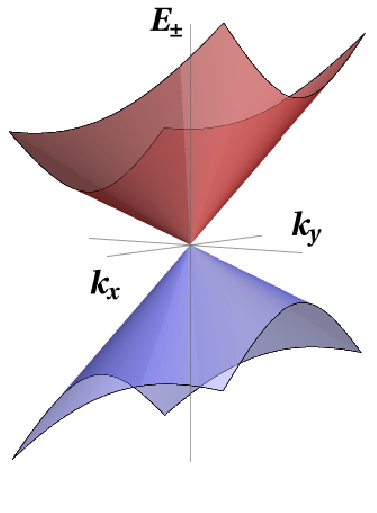
\includegraphics[width = 0.23 \textwidth]{disp}} \hspace{4 cm}
\subfigure[]{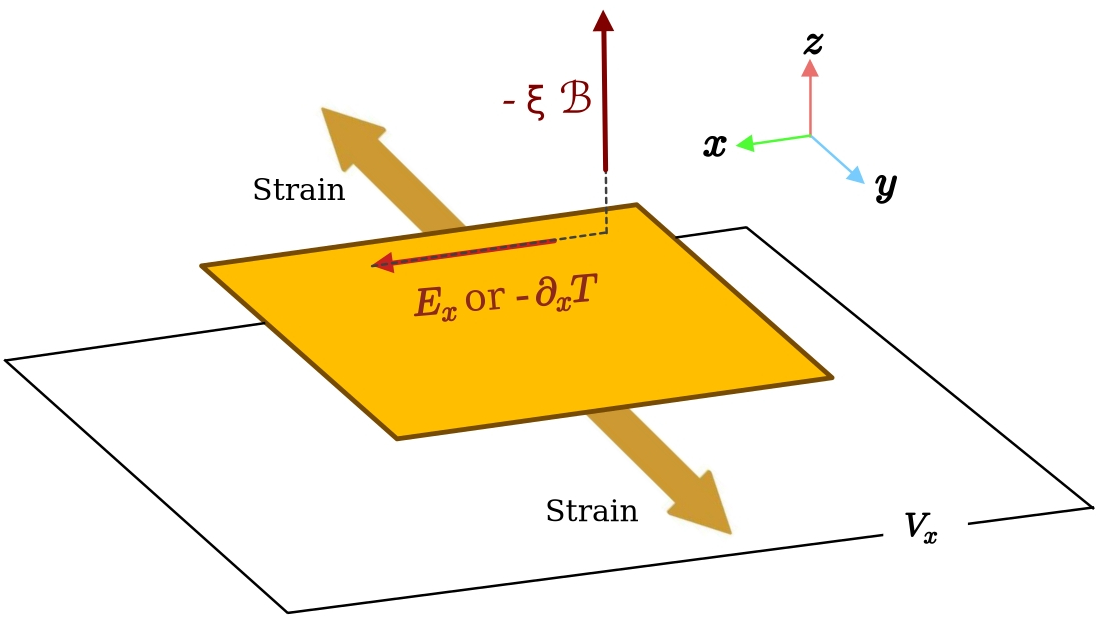
\includegraphics[width=0.5\textwidth]{EB}}
\caption{\label{figdis}(a) Energy bands for a tilted Dirac cone. (b) Set-up to measure the longitudinal transport coefficients in the presence of a strain-induced pseudomagnetic field. Here, a uniform and time-independent electric field ($E_x$) or temperature gradient ($- \,\partial_x T$) is applied in the $x$-direction and $V_x$ is the associated voltage.}
\end{figure*}
%%%%%%%%%%%%%%%%%%%%%%%%%%%%%%%%
 

 

%%%%%%%%%%%%%%%%%%%%%%%%%%%%%%%%%%%%
\section{Model}
\label{secmodel}

%%%%%%%%%%%%%%%%%%%%%%%%%%%%%%%%%%%%%%%%%%%%

The minimal low-energy effective Hamiltonian of a single tilted Dirac cone, at a valley indexed by $\xi $ (where $\xi =\pm$), is captured by Ref.~\cite{tilted-goerbig, ips_tilted_dirac}
\begin{align}
\label{eqham}
\mathcal{H}_0 =   \xi\, v_x\, k_x \,\sigma_x +    v_y \, k_y \,\sigma_y
+ \left ( \boldsymbol{v}_0 \cdot\boldsymbol{k} \right ) {\mathbb I}_{2\times 2} \,, \quad
%%%%%%%%%%%%%%%%%%%%%%%
\boldsymbol{v}_0 \equiv  
v_{0x} \,   {\boldsymbol{\hat x}} +  v_{0y} \,  {\boldsymbol{\hat y}}\,, \quad
v_{0x} \equiv   v_x\,\eta_x \, ,\quad
v_{0y} \equiv  v_y\,\eta_y \,,
\end{align}
where $\sigma_x $ and $\sigma_y $ denote the first two Pauli matrices. The velocities, $v_x$ and $v_y$, represent the components of the Fermi velocities along the $k_x$- and $k_y$-axes, respectively. Finally, the amount of tilt with respect to these two axes
are parametrised by $\eta_x$ and $\eta_y$, respectively. Clearly, the tilt introduces diagonal terms in the $2\times 2$ Hamiltonian, which did not exist in the untilted Dirac cone case.
In the following, we will use the indices $\lbrace i, \, j \rbrace $ to label the component of a vector (or tensor) along the $
\lbrace i^{\rm th}, \, j^{\rm th} \rbrace$ Cartesian coordinate.


Here, we restrict ourselves to the cases when $ \eta <1$, where $\eta  \equiv \sqrt{ {\eta_x}^2 + {\eta_y}^2  }$, which implies that we are going to consider the type-I (or undertilted) phases, where the 1d Fermi surfaces at finite values of the chemical potential ($\mu$) are closed, i.e., ellipses. The energy eigenvalues of the two-band Hamiltonian are:
\begin{align}
E_{\pm} ({\boldsymbol k}) = (\boldsymbol{v}_0 \cdot \boldsymbol{k} )
 \pm \, \epsilon_k \,, \text{ where } 
\epsilon_k = \sqrt{ v^2_x \, k^2_x + v^2_y \, k^2_y } \,.
\end{align}


%%%%%%%%%%%%%%%%%%%%%%%%%%%
\subsection{Incorporating strain}

%The momentum-space Hamiltonian in the vicinity of a Dirac cone, containing only nn hoppings, can be expressed as
%\begin{align}
%& H_d = -\, t \sum_{\bs k} \sum \limits_{ \lbrace \bs M_\alpha \rbrace } \left[ 
%e^{ -\, i \, \bs k \cdot \bs M_\alpha} \, a_{\bs k}^\dagger \, b_{\bs k}
%+ 
%e^{  i \, \bs k \cdot \bs M_\alpha} \, b_{\bs k}^\dagger \, a_{\bs k}
%\right ], \quad \alpha \in \lbrace 1, \,2 ,\, 3 \rbrace \,,\nn
%%%%%%%%%%%%%
%& \bs M_1 = a_0 \, \bs{\hat y}\,, \quad \bs M_2 = - \frac{a_0}{2} \left(\sqrt 3 \,\bs{\hat x} + \bs{\hat y}\right),
%\quad \bs M_2 =  \frac{a_0}{2} \left(\sqrt 3 \,\bs{\hat x} - \bs{\hat y}\right).
%\end{align}
%Here, $a^\dagger _{\bs k}$ and $b ^\dagger _{\bs k}$  stand for the creation operators associated with the A and B sublattice degrees of freedom, respectively. The set $\lbrace \bs M_\alpha \rbrace$ denotes the nn-vectors for hoppings between the nn sublattices.



The real-space Hamiltonian in the vicinity of a Dirac cone, containing only nearest-neighbour (nn) hoppings, can be expressed as
\begin{align}
\label{eqnn}
& H_d = -\, t \sum_{\bs r_A} \sum \limits_{ \lbrace \bs M_\alpha \rbrace } \left[ 
a_{\bs r_A}^\dagger \, b_{\bs r_A + \bs M_\alpha} + b_{\bs r_A + \bs M_\alpha }^\dagger \, a_{\bs r}
\right ], \quad \alpha \in \lbrace 1, \,2 ,\, 3 \rbrace \,,\nn
%%%%%%%%%%%%
& \bs M_1 = a_0 \, \bs{\hat y}\,, \quad \bs M_2 = - \frac{a_0}{2} \left(\sqrt 3 \,\bs{\hat x} + \bs{\hat y}\right),
\quad \bs M_3 =  \frac{a_0}{2} \left(\sqrt 3 \,\bs{\hat x} - \bs{\hat y}\right),
\end{align}
where $a^\dagger_{\bs r}$ and $b ^\dagger _{\bs r}$ stand for the creation operators associated with the A and B sublattice sites, respectively, which are separated by the nn-distance $a_0$. The discrete coordinate-locations, $\bs r_A$ denote the A-sublattice sites and the set $\lbrace \bs M_\alpha \rbrace$ represents the nn-vectors for hopping between the nn sublattice-sites. We use the effective forms derived in Refs.~\cite{neto-strain-graphene, strained-dirac-franz} for a Dirac cone subjected to uniaxial strain, which produces the pseudomagnetic fields that we want to analyze in this paper. In this procedure, the uniaxial strain pattern is incorporated in the system through a modulation of the nn hoppings into a  smooth function of the spatial coordinates. For the positions $\bs r_A $ and $\bs r_a + \bs M_\alpha $, the hopping amplitude is given the form of 
\begin{align}
t \rightarrow t_{\alpha}(\bs r_A) 
 = t_\alpha\, e^{-\gamma \,\Delta u_\alpha }
=  t  \left ( 1 -  \gamma_a \right)
 + \order{ \gamma _\alpha^2 } \,, \quad \gamma_\alpha \equiv \gamma\, \Delta u_\alpha, 
\end{align}
which depends on a displacement, $ \Delta u_{\alpha}$, along the three nn-bond directions. We assume the original displacement-field is $\bs u (\bs r) = u_x (\bs r)  \, \bs {\hat x} + u_y (\bs r) \, \bs {\hat y}$, such that $\bs u ({\bs r_A} + {}\bs M_\alpha) - \bs u (\bs r_A) = \Delta u_\alpha $, which we postulate to be of small magnitude (such that $\gamma_\alpha \ll 1 $).
Next, we are interested in a configuration of the strain tensor, $\varsigma_{ij}$, such that only its $\varsigma_{yy}$-component survives (i.e., $ \varsigma_{xx} = \varsigma_{xy} = \varsigma_{yx} = 0 $), which is purely $y$-dependent. Invoking the relation $\Delta u_{\alpha} = \sum_{i, j} \frac{ \left(M_\alpha \right)_i \left( M_\alpha\right)_j } {a_0}\,\varsigma_{ij}$, we deduce that
\begin{align}
\Delta u_1 = 4\, \Delta u_2 = 4 \, \Delta u_3 = a_0\, \varsigma_{yy}  (y)\,.
\end{align}



Although the authors in Ref.~\cite{strained-dirac-franz} derived the strain-induced terms for untilted isotropic Dirac cones, initially located at the $K$ and $K^\prime $ corners of graphene's BZ, we assume that this applies also to the case of the tilted versions (shifted away from the high-symmetry points). \rd{This is motivated by the observation that} the Dirac-point and the $K$-point of the deformed
lattice do not coincide in general Ref.~\cite{neto-strain-graphene}, which can be attributed to the fact that the applied strain not only affects the hoppings but also causes a distortion of the lattice itself. We just need to ensure that the strain to be applied in such a way that it affects mainly the off-diagonal terms arising from the nn hoppings. Therefore, in the vicinity of a Dirac-point hosting a tilted cone with anisotropic Fermi velocities as well, the applied strain modifies the continuum version of the low-energy Hamiltonian to Refs.~\cite{strained-dirac-franz, complex-LL-strained-graphene}
%%%%%%%%%%%%%%
\begin{align}
\label{eqhtot}
& \mathcal H_\xi (k_x, y) = \left[ 
\left(v_x \, \eta_x \, k_x + v_y \,\eta_y\, k_y \right)  {\mathbb I}_{2\times 2} 
+ \mathcal{H}_s(y; k_x, k_y) \right ]\big \vert_{k_y \rightarrow -i\, \partial_y}
\,, \quad 
\mathcal{H}_s  = v_x \, d^\xi_x (\bs k)\,\sigma_x + v_y\,d^\xi_y (\bs k)\,\sigma_y  \,, \nn &
%%%%%%%%
\nn & d^\xi_x(\boldsymbol{k}) = \xi \left( \left (1 - \frac{ \tilde \gamma} {4}\right ) {k}_x 
+\, \xi \, \frac{ \tilde \gamma} {2\, a_0}\right)  \,,
%%%%%%%%%
\quad  d^\xi_y(\boldsymbol{k}) =
\left (1 - \frac{3\, \tilde \gamma } {4} \right )  k_y 
+ \xi\, a_0\,\frac{ k_x \, k_y}{2} \left (1 - \frac{\tilde \gamma} {4}  \right ) ,
%%%%%%%%
\quad \tilde \gamma = \gamma\,a_0 \, \varsigma_{yy}\,.
\end{align}
%%%%%%%%%%%%%%%%%%%%%%%%%%%%%%%
Here, the index $\xi =\pm$ labels two inequivalent valleys. In this paper, we will consider tilt with respect to the $k_x$-axis only, setting $\eta_y = 0 $.

{\color{red}
\label{secvalid}
We make the assumptions behind Eq.~\eqref{eqhtot} explicit. The tilt originates from the nnn hoppings, which connect sites of the same sublattice and therefore contribute, at linear order in the momentum, only to the term proportional to the identity matrix. The strain-induced terms originate from the modulation of the nn hoppings, which connect the two sublattices and therefore enter the off-diagonal part $\mathcal H_s$. At the order retained, the two sets of terms are additive provided that two conditions hold. The first is that the strain dependence of the nnn hoppings is neglected, which changes the tilt only by a relative amount of order $\tilde\gamma$ times the ratio of the nnn and nn hoppings, and this is small within the regime of validity stated below. The second is that the off-diagonal part is expanded around the Dirac point with the coefficients appropriate to the nn hopping. This second condition is not rigorous for a Dirac point displaced from $K$, because the numerical coefficients of the terms of order $a_0\,k$ in $d^\xi_x$ and $d^\xi_y$ then differ from those obtained by expanding around $K$, by amounts of the order of the displacement. We have not derived the corrected coefficients for a specific lattice. Eq.~\eqref{eqhtot} is therefore adopted as a model for the coupling of tilted cones to strain, and we do not claim that it follows from a first-principles calculation for a particular material. The terms of order $a_0\,k_x$ matter for the results, since they are responsible for the intrinsic dispersion of the PLLs discussed in Sec.~\ref{secll}. The dispersion caused by the tilt does not depend on them. Statements on the lattice-induced part of the dispersion should be understood as statements of the model, and their material-specific values require the corresponding coefficients of the lattice in question.

The strain configuration is the following. Only the component $\varsigma_{yy}$ is nonzero, and it varies linearly along $y$. This describes a uniaxial strain along the direction of the bond $\bs M_1$ with a constant gradient along the same direction, which modulates the three nn hoppings in the ratios $\Delta u_1=4\,\Delta u_2=4\,\Delta u_3$. Other orientations, and shear components, generate different components of the pseudogauge field and are not covered by Eq.~\eqref{eqhtot}. We restrict the tilt to the $k_x$-axis for a technical reason. For $\eta_y\neq0$, the term $v_y\,\eta_y\,k_y$ turns into $-i\,v_y\,\eta_y\,\partial_y$, and the equation for $\phi_B$ becomes a pair of coupled equations for its real and imaginary parts, which we could not solve analytically. Results for an arbitrary direction of the tilt are therefore not available in this work.

The expansion leading to Eq.~\eqref{eqhtot} is controlled when $|\tilde\gamma|\ll1$ and $a_0\,|k_x|\ll1$. Since $\tilde\gamma=\gamma\,a_0\,\varsigma_{yy}$ and $\varsigma_{yy}=2\,b\,y/\gamma$, the first condition reads
\begin{align}
|\tilde\gamma|=\gamma\,a_0\,|\varsigma_{yy}|=2\,a_0\,e\,|\mathcal B|\,|y|\ll1\,,
\end{align}
and it restricts the strain to $|\varsigma_{yy}|\ll1/(\gamma\,a_0)$ in the region occupied by the states. For graphene, $\gamma\,a_0$ is of the order of 2 to 3, and strains of a few per cent keep $|\tilde\gamma|$ below $0.1$. For a strained region of width $W$, the PLL states must fit into the region, which requires $\ell_{\mathcal B}=1/\sqrt{e\,|\mathcal B|}\ll W$. The condition above, evaluated at $|y|\sim W$, requires $e\,|\mathcal B|\ll1/(2\,a_0\,W)$. Both conditions are fulfilled together if
\begin{align}
\frac{1}{W^2}\ll e\,|\mathcal B|\ll\frac{1}{2\,a_0\,W}\,.
\end{align}
For $W=100$ nm and $a_0=0.142$ nm, this window corresponds to $0.07\ {\rm T}\ll|\mathcal B|\ll23\ {\rm T}$ in conventional units. The condition $a_0\,|k_x|\ll1$ limits the part of the spectrum that can be trusted. The levels with large $n$, and the portions of each level with large $|k_x|$, lie beyond it. In particular, the finite upper bound on $n$ in Eq.~\eqref{eqevals} indicates the loss of validity of the continuum model. For levels close to this bound, the spatial extent of the states reaches values for which $|\tilde\gamma|$ is of order unity. The results of this work should therefore be read as results for the low-lying PLLs, that is for $n$ well below the upper bound and for $a_0\,|k_x|\ll1$.
}

{\color{red}
Notation: the symbol $\varsigma_{ij}$ denotes the strain tensor, of which only $\varsigma_{yy}$ is nonzero. The pseudomagnetic field is denoted by $\mathcal B$ throughout, and a real magnetic field does not appear in this work. We also use $b=e\,\mathcal B$ and $\zeta=e\,\mathcal B\,v_y/v_x$. The latter must not be confused with $\varsigma_{yy}$. The dimensionless variables carrying a tilde are defined in Sec.~III.
}




We observe that the $\varsigma_{yy}$ terms couples to the $k_x$ terms in a way such that the coupling of fermions with the effective pseudogauge-field component, $ \xi\, e \,  \mathcal{A}_x = \xi \, \tilde \gamma /(2\, a_0) = \xi\, \gamma \, \varsigma_{yy} / 2 $ (because, a gauge-field coupling is obtained by the substitution $k_x \rightarrow k_x - \text{charge } \times \mathcal{A}_x $). Thus, $ \mathcal{A}_x $ appears with opposite signs for $ D$ and $D^\prime$. In addition, we find that $\varsigma_{yy}$ also renormalizes the values of the Fermi velocities. For a clearer visualization of the gauge-field coupling, remembering that $  
\tilde \gamma  = 2\, a_0 \,e \,  \mathcal{A}_x $, we rewrite the Hamiltonian with
%%%%%%%%%%%%%%%%%%%%%%%%%%
\begin{align}
 & d^\xi_x(\boldsymbol{k}) = \xi  \left (1 - \frac{ a_0 \,e \,  \mathcal{A}_x} {2}\right ) {k}_x 
+  \xi^2\,  e \,  \mathcal{A}_x  \,,
%%%%%%%%%
\quad d^\xi_y(\boldsymbol{k}) =
\left ( 1- 2\,a_0 \,e \,  \mathcal{A}_x  +  \frac{ \xi^2 \,a_0 \,e \,  \mathcal{A}_x} {2} 
\right )  k_y 
+  a_0\,\frac{ \xi\,k_x \, k_y}{2} \left (1 - \frac{ a_0 \,e \,  \mathcal{A}_x} {2}  \right ) \nn
%%%%%%%%%%%%%%%%%%%%%%%%%%%%%%%% next line 
%%%%%%%%%%%%%%%%%%%%%%%%%%%%%%%%%%
\Rightarrow & \; d^\xi_x(\boldsymbol{k}) = \xi  \,\Pi_x
  - \xi\,k_x  \frac{ a_0 \,e \,  \mathcal{A}_x} {2} \,,
%%%%%%%%%
\quad d^\xi_y(\boldsymbol{k}) =
\left ( 1- 2\,a_0 \,e \,  \mathcal{A}_x \right )  k_y  
+  \frac{ a_0\,\xi \, k_y} {2} \,\Pi_x \,,
\text{ where } \Pi_x =  k_x +  \xi \,  e \,  \mathcal{A}_x \,.
\end{align}
%%%%%%%%%%%%%
We find that a direct interpretation of the Hamiltonian as an analogy of actual LLs is a bit problematic because we have a mix of both $\Pi_x$ and $k_x $ terms. There has been the interpretation of the extra factors as a modulation of the Fermi velocities Ref.~\cite{complex-LL-strained-graphene}, but we will take the point of view of solving for the energy levels of the resulting system and work out its eigenspectra, which we will call as the PLLs.


By taking $\mathcal{A}_x = \, y\, {\mathcal B} $ (analogue of the Landau gauge), we can engineer $\bs{\mathcal B}= \nabla_{\bs r} \cross \bs{\mathcal A }$ to be directed perpendicular to the plane of the 2d lattice, which we call the negative $z$-direction. Therefore, we define
\begin{align}
 \varsigma_{yy} = \frac{2 \, b\, y} {\gamma} \,, \quad
b = e\, \mathcal B\,,
\end{align}
we generate $ \bs{\mathcal B} = -\,{\mathcal B} \, \bs{\hat z}$, which acts on the two valleys with opposite signs. Because of breaking the translation symmetry along the $y$-direction, $k_y $ is no longer a good quantum number, and we are forced to work in a hybrid spatial-momentum coordinates (viz. $y$ and $k_x$). Overall, our system acquires anisotropy from three ingredients: (i) $ v_x \neq v_y$; (ii) uniaxial strain; (iii) tilting. 

%%%%%%%%%%%%%%%%%%%%%%%%%%%%%%%%
\begin{figure*}[t!]
\centering
%\subfigure[]{\includegraphics[width= 0.6 \textwidth]{figPLL-notilt}}
\subfigure[]{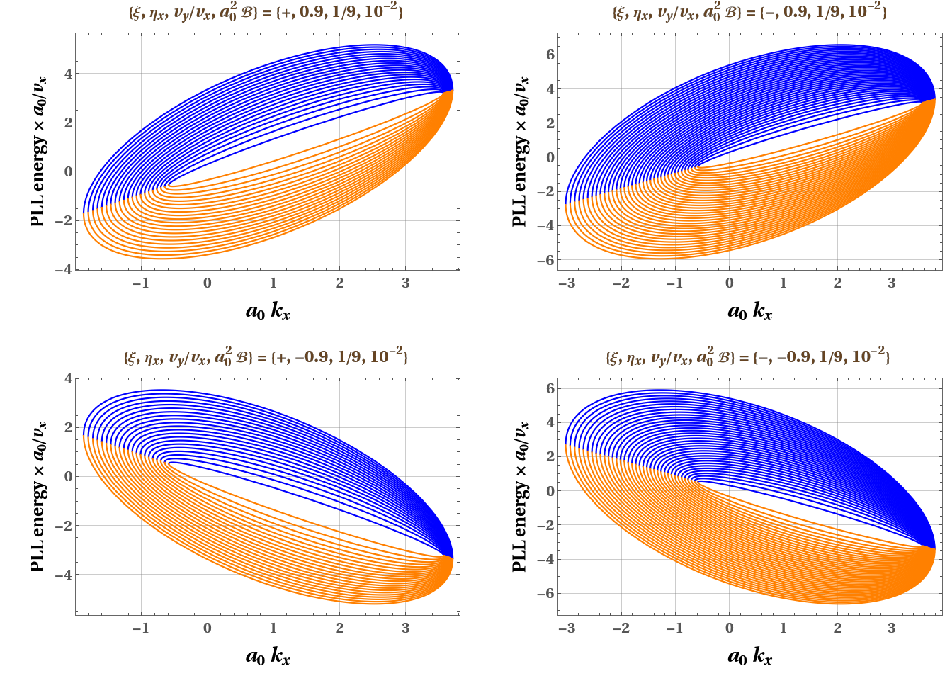
\includegraphics[width= 0.7 \textwidth]{figPLL}}
\subfigure[]{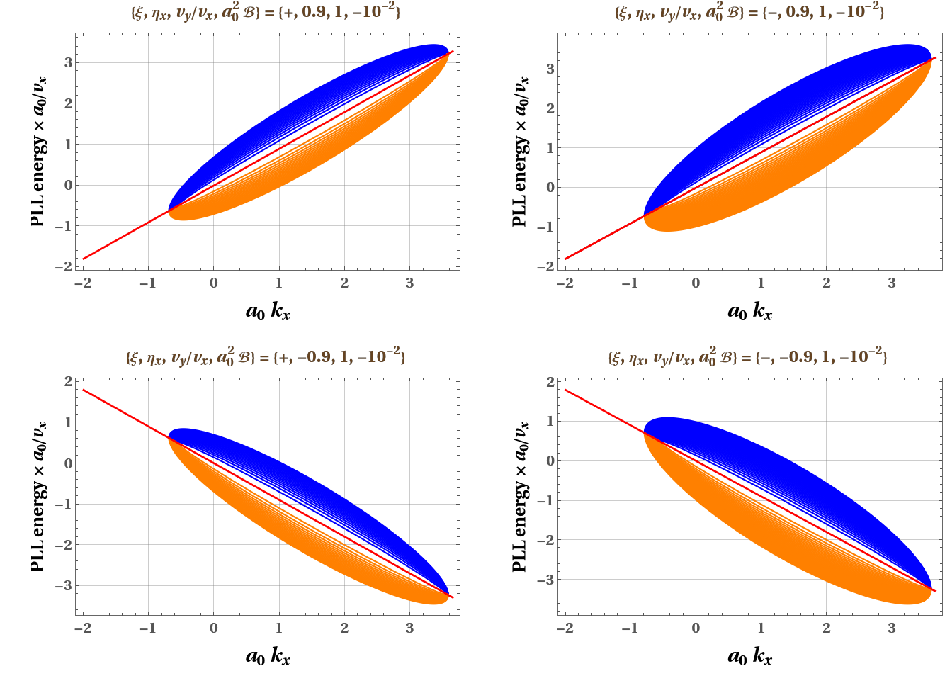
\includegraphics[width= 0.7 \textwidth]{figPLL2}}
\caption{Dispersion of the PLLs for some chosen parameters shown in the plot-labels. \rd{The valley is $\xi=+$ in all panels.}\label{fig:spectrum_B}}
\end{figure*}




%%%%%%%%%%%%%%%%%%%%%%%%%%%%%%%%
\subsection{Pseudo-Landau levels}
\label{secll}

%%%%%%%%%%%%%%%%
\begin{figure*}[th!]
\centering
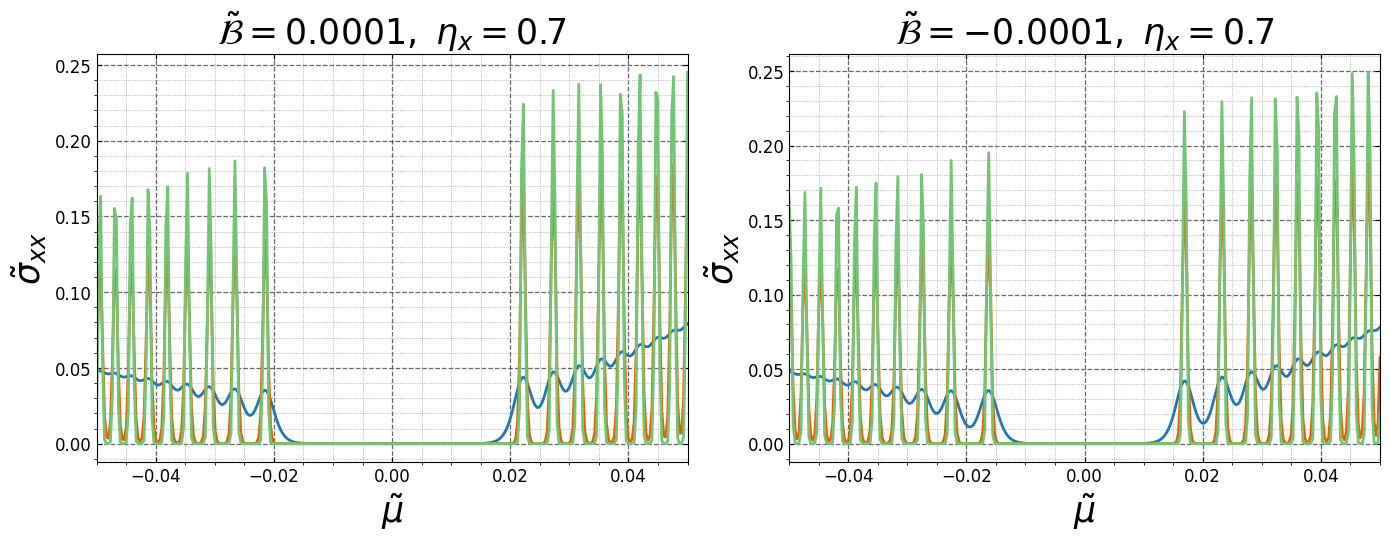
\includegraphics[width= 0.7 \textwidth]{sigma}
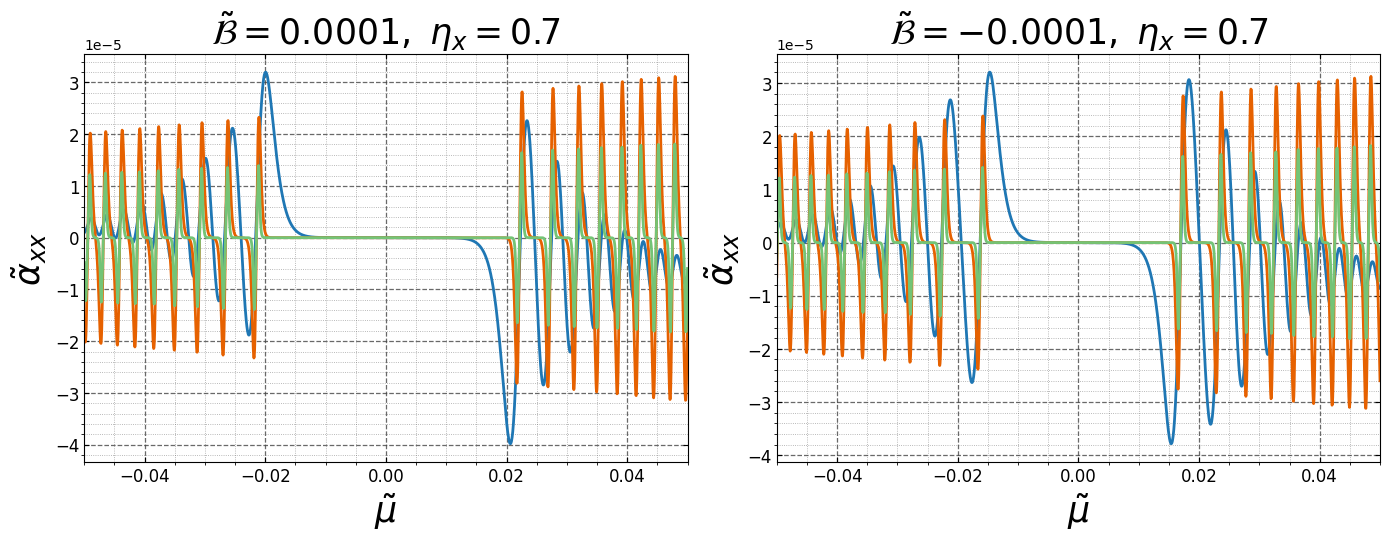
\includegraphics[width=0.7\textwidth]{alpha} 
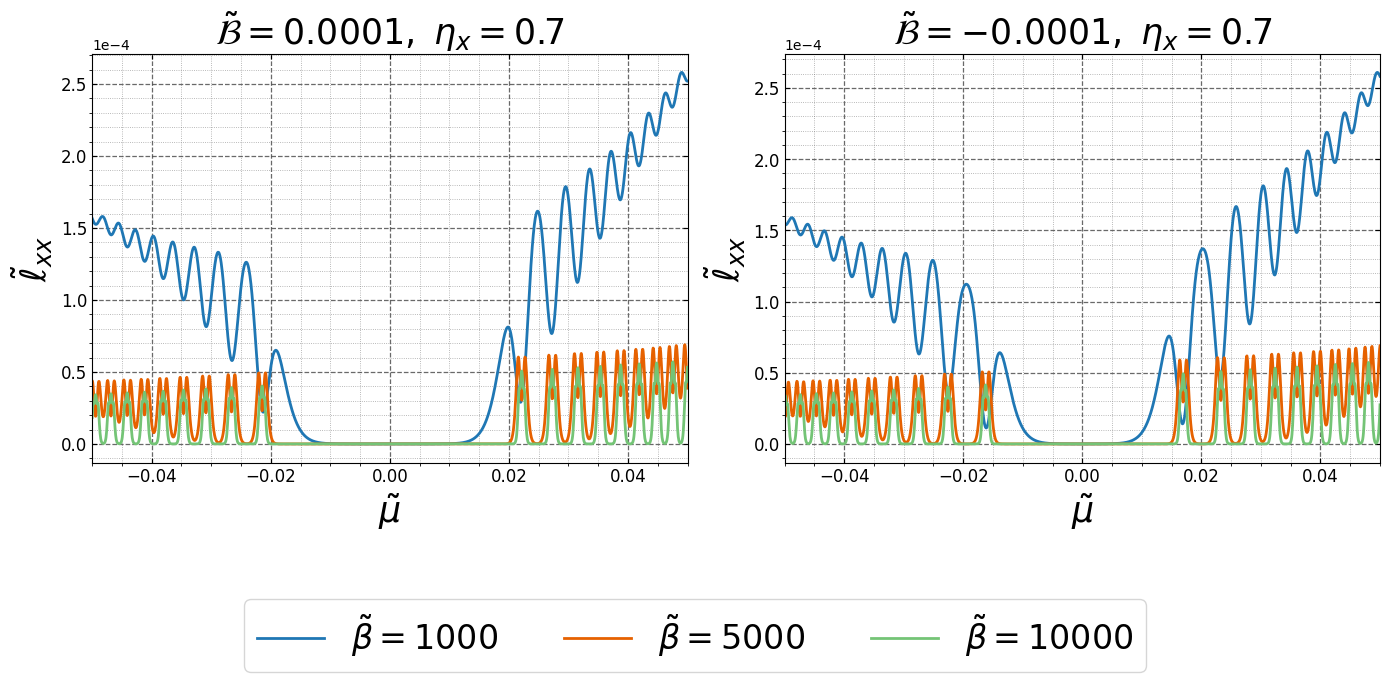
\includegraphics[width=0.7\textwidth]{ell}
\caption{Linear-response coefficients $\tilde \sigma_{xx}$, $\tilde \alpha_{xx}$, and $\tilde \ell_{xx}$, as functions of $\tilde \mu$. We have plotted them for 3 different values of $\beta $. We have taken $v_y/ v_x = 0.8 $. \rd{The quantities are defined in Sec.~III, and they are normalised by $\tau$. }\tbd{Parameters to be completed from the plotting scripts: values of $\tilde{\mathcal B}$, $\eta_x$ and $\tilde\beta$ not stated above. The valley is $\xi=+$.}\label{fig:transport}}
\end{figure*}
%%%%%%%%%%%%%%%%%%%

%%%%%%%%%%%%%%%%
\begin{figure*}[t!]
\centering
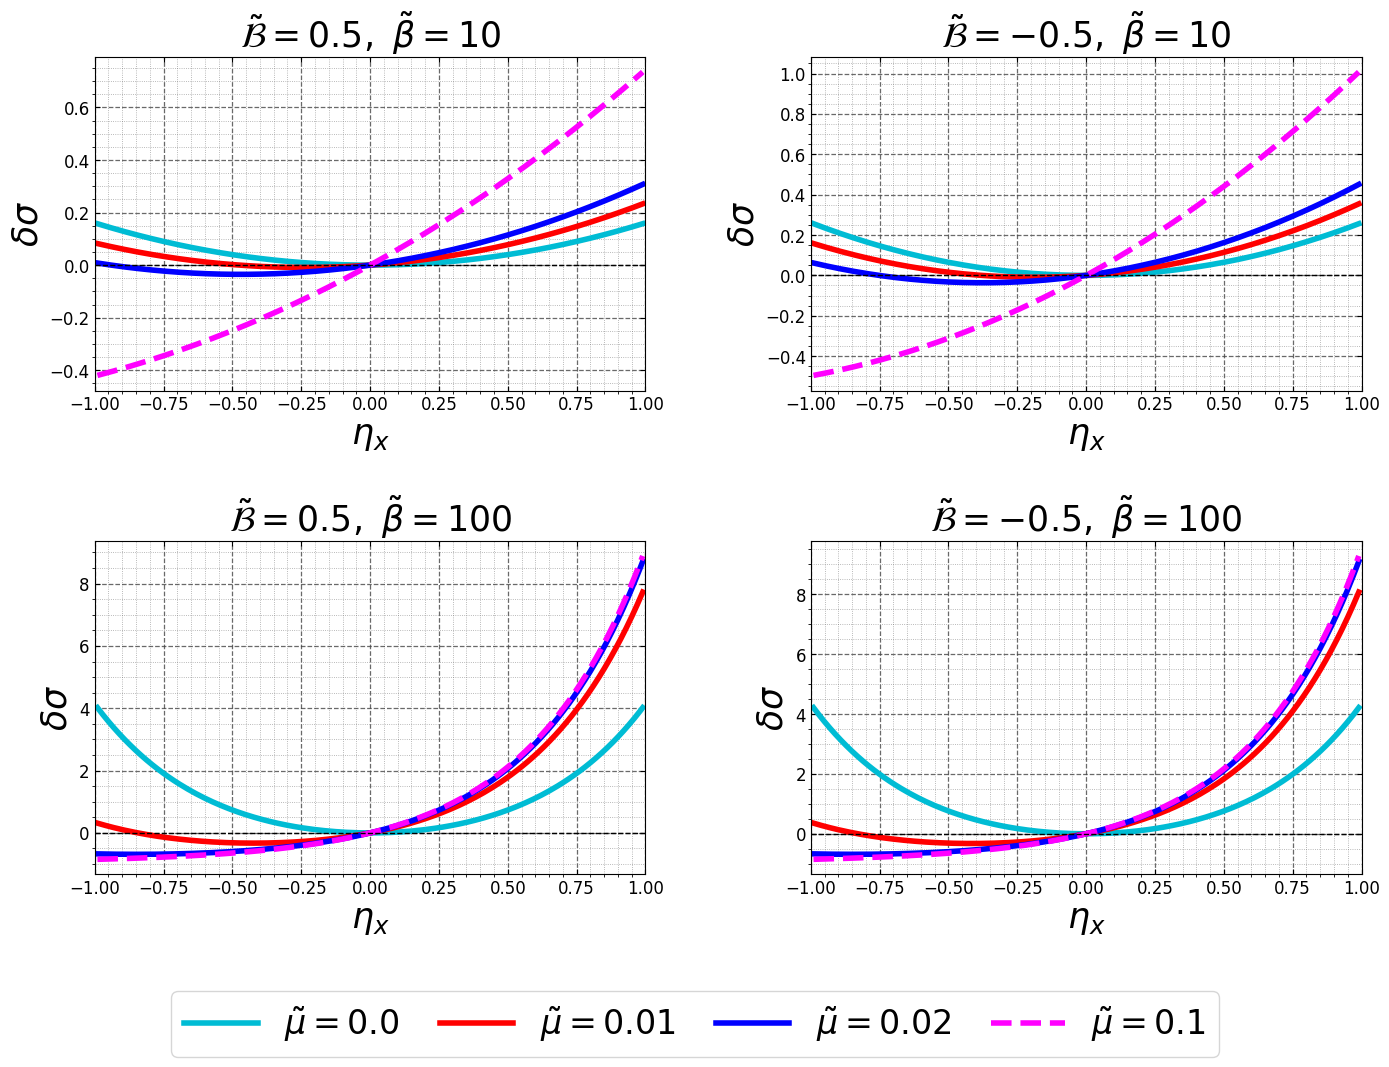
\includegraphics[width= 0.7 \textwidth]{sigma_etax1}
\caption{Variation of electrical conductivity with $\eta_x$ by setting $v_y/ v_x$ to $ 0.8 $. Here, $ \delta \sigma \equiv \sigma_{xx}  (\eta_x)/ \sigma_{xx} (\eta_x=0) -1 $. \rd{The valley is $\xi=+$, and the remaining parameters are fixed at the values stated in the panel.} \tbd{Parameters to be completed from the plotting scripts: values of $\tilde{\mathcal B}$, $\eta_x$ and $\tilde\beta$ not stated above. The valley is $\xi=+$.}\label{figsigeta}}
\end{figure*}
%%%%%%%%%%%%%%%%%%%



To find the solution for the PLLs of the full Hamiltonian in Eq.~\eqref{eqhtot}, we need to solve for the eigenvalue equation,
\begin{align}
\mathcal{H}_{\xi} \,\Phi (k_x, y) = E \,\Phi (k_x, y)\,,\quad
\Phi^T (k_x, y) = \begin{bmatrix}
\phi_A (k_x, y) & \phi_B(k_x, y) 
\end{bmatrix} .
\end{align}
%%%%%%%%%%%%%
Since $k_x$ remains a good quantum number (because of unbroken translation symmetry along the $x$-direction), we work with the momentum-variable for the $x$-direction. The steps for solving the coupled differential equations involving the unknowns, $\phi_A$ and $\phi_B$, are detailed in the Appendix. Following those intermediate steps, we get the PLLs as
%%%%%%%%%%%%%%%%%%%
\begin{align}
& \frac{  E^{\xi}_{n, \rm{si}} (k_x, \mathcal B) } {v_x} =  
\eta_x \,   k_x
% +  \text{si} \, \tilde E^\xi_n (k_x) \,, 
%%%%%%%%%%%%
%\quad \tilde E^\xi_n (k_x) =  
+ \,\sqrt{\tilde r_\xi^2 \, \left( |\zeta | \, n
+ \frac{e \, \mathcal B+|\zeta|}{2} \right)^2
+ \left (k_x \, \tilde r_\xi + s_{-\xi} \, s_\xi \right )
\left (2 \, |\zeta |\, n + e \, \mathcal B+|\zeta| \right )}  \,,\nn
%%%%%%%%%%%%%%%%%%%%%%%%%%%%%%%%%%%
& \text{ where } \text{si} = \pm \,, \quad
s_\xi = 1 + \frac{\xi \, k_x\, a_0 } {2}\,, \quad
r_\xi = \frac{3}{2} + \frac{\xi \, k_x\, a_0 } {4}\,,\quad
\tilde{r}_\xi = a_0 \, r_\xi  \,, \quad \zeta =  e \, {\mathcal B} \, \frac{v_y}{v_x}\,,
%%%%%%%%%%%
\nn & \text{and } n \in \left\{ 0, \,1, \, 2,\cdots, 
\left\lfloor\frac{8 \,(2  + 3 \, \xi \,a_0\, k_x)}   { a_0^2\,|\zeta| \,(6 +\xi \,a_0\,  k_x)^2} \right\rfloor \right\}.
\label{eqevals}
\end{align}
%%%%%%%%%%%%%%%%%%%%%%%%
We have labelled them by the integer-index $n$, momentum $k_x$, and band-index $\pm$ at the valley $\xi$. 
In the above expression, the symbol $\left \lfloor  \Upsilon \right \rfloor$ denotes the greatest integer less than or equal to $\Upsilon$.
We get an upper-bound for the number of PLLs that depends on strain induced through the pseudo magnetic field in the system. For small $ |\mathcal{B}| $, the expression approximates to
%%%%%%%%%%%%%%%%%%%%%%%%%
\begin{align}
\frac{ E^{\xi}_{n, \rm{si}} (k_x, \mathcal B) } {v_x} \simeq    \eta_x \,   k_x 
+ \text{si}\, \sqrt{\left (k_x \, \tilde r_\xi + s_{-\xi} \, s_\xi \right )
\left (2 \, |\zeta |\, n + e \, \mathcal B+|\zeta| \right )} .
\end{align}
Since $n\in \lbrace 0 \rbrace \cup \mathbb{Z}^+$, with an upper-bound of $
\left\lfloor\frac{8 \,(2  + 3 \, \xi \,a_0\, k_x)}   { a_0^2\,|\zeta| \,(6 +\xi \,a_0\,  k_x)^2} \right\rfloor$, we have a restricted number of PLLs. For positive values of $\eta_x$, it is possible for $E^\xi_{n, -} (k_x, \mathcal B)$
to take negative values as well. This happens when $ \eta_x \, a_0 \,  k_x  > \sqrt{\left (k_x \, \tilde r_\xi + s_{-\xi} \, s_\xi \right )
\left (2 \, |\zeta |\, n + e \, \mathcal B + |\zeta| \right )} $. Similarly, for $\eta_x<0$, we end up with negative values for $ E^\xi_{n, +}
( k_x, \mathcal B )$ as well.


%%%%%%%%%%%%%%%%
\begin{figure*}[t!]
\centering
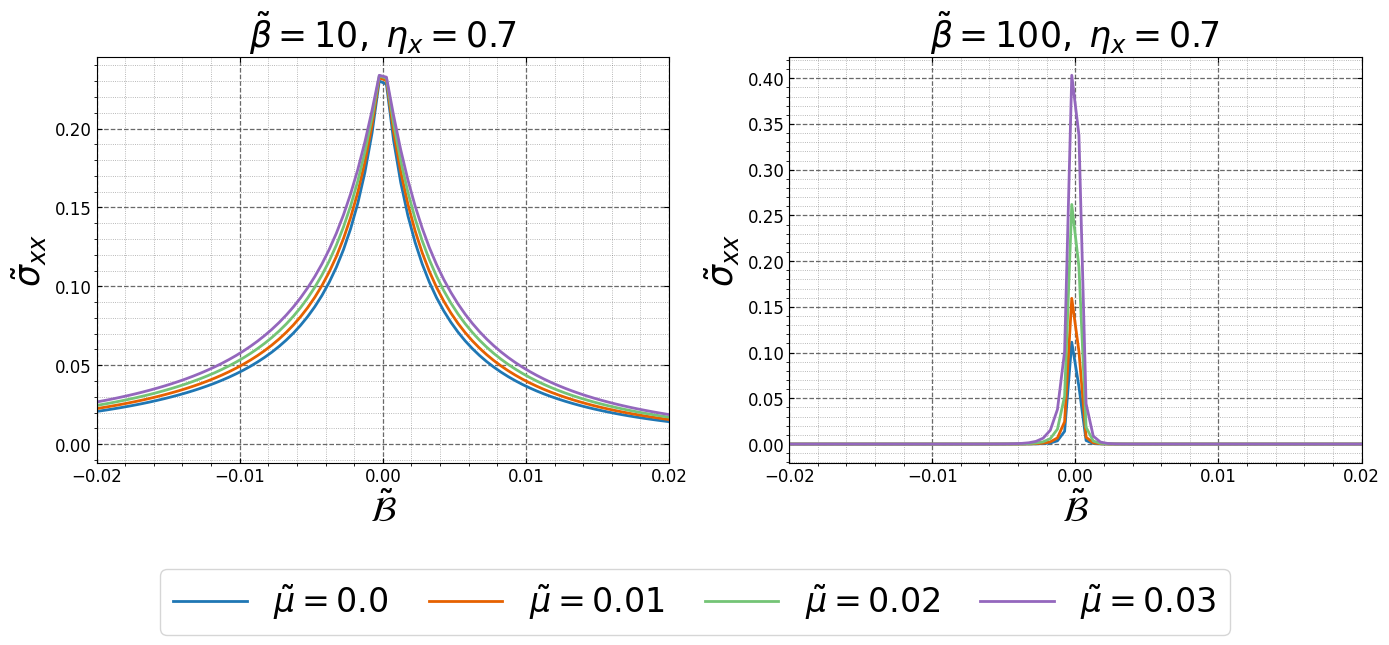
\includegraphics[width= 0.7 \textwidth]{sigma_B}
\caption{Variation of electrical conductivity with $\mathcal B$. \rd{The plotted quantity is $\tilde\sigma_{xx}=L_y\,\sigma_{xx}/(\tau\,v_x)$ as a function of $\tilde{\mathcal B}=a_0^2\,\mathcal B$.} \tbd{Parameters to be completed from the plotting scripts: values of $\tilde{\mathcal B}$, $\eta_x$ and $\tilde\beta$ not stated above. The valley is $\xi=+$.}\label{figsigB}}
\end{figure*}
%%%%%%%%%%%%%%%%%%%


We represent the unique features of the PLLs by Fig.~\ref{fig:spectrum_B} for some representative parameter values. There, we observe the dispersive Landau levels, where the $\eta_x$-dependent term causes a tilt in the overall spectrum.
The most intriguing nature that is revealed comprises the PLLs forming closed curves rather than dispersing out indefinitely as $ |k_x|$ is cranked up. Of course there also exists a lone PLL in the form of a line (not closed) --- this one represents a non-dispersive or flat band in the absence of tilting [cf. the red lines in Fig.\ref{fig:spectrum_B}(b)]. Furthermore, the range of PLL-curves are more expanded for the $D$-valley compared to the $D^\prime$-valley, showing that the system is not valley-symmetric --- this is a consequence of the shifting of the Dirac points under strain.

{\color{red}
The physical content of Eq.~\eqref{eqevals} can be summarised as follows. For $\xi=+$ and small $\mathcal B$, the levels are
\begin{align}
\frac{E^{+}_{n,\rm si}}{v_x}\simeq\eta_x\,k_x+{\rm si}\,\sqrt{\left(1+\frac{3\,a_0\,k_x}{2}\right)\left(2\,|\zeta|\,n+e\,\mathcal B+|\zeta|\right)}\,.
\end{align}
At $k_x=0$ and for $n\gg1$, this reduces to the anisotropic Dirac ladder $\sqrt{2\,n\,v_x\,v_y\,e\,|\mathcal B|}$. Four ingredients are encoded in the full expression. First, the term $\eta_x\,k_x$ is a rigid tilt of all levels. It multiplies the identity matrix, and therefore changes neither the eigenfunctions nor the number of states per level, but it gives every level the group velocity $v_x\,\eta_x$ in addition to that of the untilted dispersion. Second, the factor $1+3\,a_0\,k_x/2$ stems from the strain-induced renormalisation of the velocities and from the terms of order $a_0\,k_x$ of the lattice, and it produces the dispersion of the untilted PLLs. Third, the valley index enters through $s_\xi$ and $r_\xi$, which is the origin of the valley asymmetry visible in Fig.~\ref{fig:spectrum_B}. Fourth, the index $n$ has a finite upper bound, whose meaning is discussed in Sec.~\ref{secvalid}.

The PLLs are normalisable bound states, and not artefacts of the hybrid representation. Since the strain depends only on $y$, translation invariance along $x$ is intact and $k_x$ is a good quantum number, while the $y$-dependence is solved exactly in the Appendix. The eigenfunctions are generalised Laguerre polynomials multiplied by exponentially decaying factors. They vanish at the singular point $y=y^\xi_{\rm sg}$, where the coefficient of $k_y$ in $d^\xi_y$ vanishes, and they are localised in $y$ over a length of the order of $\ell_{\mathcal B}$ around a centre that depends on $k_x$. In the semiclassical picture, they correspond to cyclotron-like orbits whose guiding centre drifts along $x$ with the group velocity $v^{\xi,{\rm si}}_x(n;k_x)$ [Eq.~\eqref{eqgv}]. In a uniform real field, the energy of a level does not depend on $k_x$, because the translation of the guiding centre along $y$ is a symmetry. The strain does not have this symmetry. The local hopping amplitudes, and with them the local velocities, vary with $y$, and the energy of a state depends on where along $y$ it is located, that is on $k_x$. The PLLs are therefore dispersive even without tilt, and this part of the dispersion is a lattice effect of order $a_0\,k_x$. This is why the bulk longitudinal conductivity can be nonzero. At $T=0$, the electrical conductivity of a valley is
\begin{align}
\sigma^\xi_{xx}=\frac{e^2\,\tau}{L_y}\sum_{n,\,{\rm si}}\sum_{k_{\rm F}}\frac{|v^{\xi,{\rm si}}_x(n;k_{\rm F})|}{2\,\pi}\,,
\end{align}
where the sum over $k_{\rm F}$ runs over the Fermi points of each band. Every dispersive level that crosses the chemical potential contributes, while flat levels, for which $v_x=0$, do not.
}




%%%%%%%%%%%%%%%%%%%%%%
\section{Transport Properties within the semiclassical Boltzmann formalism}


Having established the pseudo-Landau level (PLL) spectrum for tilted Dirac cones under strain, we now investigate the resulting transport properties within the semiclassical Boltzmann formalism. Unlike conventional Landau levels, the PLLs obtained here are apart from being dispersive are tilted as well in momentum $k_x$, which leads to qualitatively different transport behavior in set-ups shown in Fig.~\ref{fig:transport}.
In particular, the finite dispersion of the energy spectrum ensures a non-vanishing group-velocity along the $x$-direction, in contrast to the flat Landau levels of conventional quantum Hall systems. As a result, the system exhibits finite longitudinal conductivity in the bulk. The tilting of the PLL spectra provides an extra knob to tune the qualitative nature of the bulk linear response.


%\subsection{Longitudinal linear response}

Within the semiclassical Boltzmann formalism, the longitudinal dc electrical conductivity is given by~\cite{arovas, ips-kush-review}
\begin{align}
\sigma^\xi_{xx} =  - \, \frac{e^2\,\tau} {L_y} \sum_{n, \, \text{si}} \int \frac{d k_x} {2 \,\pi}\,
\partial_{\varepsilon^{\xi, {\rm si }}_n} f_0 (\varepsilon^{\xi, {\rm si }}_n)
\, \left (\partial_{k_x }\varepsilon^{\xi, {\rm si }}_n \right)^2 ,
\end{align}
%%%%%%%%%%%%%%%%%%%%%%%%%
where $\tau$ is the relaxation time (taken to be momentum-independent in our simplified analysis), $ f_0  (\varepsilon) \equiv  \left[ e^{(\varepsilon - \mu)\,\beta} + 1\right ]^{-1} $ is the Fermi-Dirac distribution function, $ \varepsilon^{\xi, {\rm si }}_n \equiv \, 
 E^{\xi}_{n, \rm{si}} (k_x, \mathcal B)$, $\mu$ is the chemical potential, $\beta = 1/T $ is the inverse temperature, and $L_y$ is the length of the system in the $y$-direction. We take $\tau$ to be a phenomenological parameter describing various contributions to electronic scattering. The nonzero longitudinal conductivity is in stark contrast with the case of flat Landau levels, which yield vanishing longitudinal transport. 
We also compute the longitudinal thermoelectric conductivity and the longitudinal magnetothermal coefficient~\cite{arovas, ips-kush-review}, defined as
\begin{align}
\alpha^\xi_{xx} & =  \frac{e\,\tau} {L_y} \sum_{n,\,\text{si}} \int \frac{d k_x} {2 \,\pi}\,
\partial_{\varepsilon_n}  f_0 (\varepsilon^{\xi, {\rm si }}_n)\left (\partial_{k_x }\varepsilon^{\xi, {\rm si }}_n \right)^2  \frac{\varepsilon^{\xi, {\rm si }}_n - \mu}{T}
\text{ and } 
\ell^\xi_{xx} =  -\,\frac{\tau} {L_y} \sum_{n,\,\text{si}} \int \frac{d k_x} {2 \,\pi}\,
\partial_{\varepsilon^{\xi, {\rm si }}_n}  f_0 (\varepsilon^{\xi, {\rm si }}_n)\left (\partial_{k_x }\varepsilon^{\xi, {\rm si }}_n \right)^2  
\frac{ (\varepsilon^{\xi, {\rm si }}_n - \mu)^2}{T} ,
\label{eqalphaell}
\end{align}
%%%%%%%%%%%%%%%%%%%%%%%%% 
respectively.

{\color{red}
We comment on the status of this approach. Eq.~\eqref{eqalphaell} contains the intraband (Fermi-surface) contribution to the response, evaluated with the exact PLL spectrum and velocities. The effect of the quantisation on the spectrum is therefore fully retained. The semiclassical elements are the description of the scattering by a relaxation time and the neglect of the interband contributions, which involve the matrix elements of $v_x$ between different PLLs. With $\hbar=1$, these contributions are smaller than the intraband one by a factor of the order of $(\tau\,\Delta E)^{-2}$, where $\Delta E$ is the spacing between neighbouring PLLs. The approach is therefore justified when $1/\tau\ll\Delta E$ and $1/\tau\ll\mu$, which is the regime in which the PLLs are resolved. For $1/\tau\gtrsim\Delta E$, the disorder broadening merges the levels, the PLL features disappear, and the interband terms become important. Our results do not apply there. Phase-coherent effects, such as weak localisation, are not captured either.

The relaxation time is a phenomenological parameter, which we take to be independent of energy, momentum, temperature and $\mathcal B$. The plotted quantities $\tilde\sigma_{xx}$, $\tilde\alpha_{xx}$ and $\tilde\ell_{xx}$ are normalised by $\tau$, and their shapes do not depend on its value. An energy-dependent $\tau(\varepsilon)$ enters the integrals as a weight. At $T=0$, the conductivity then becomes $\sigma^\xi_{xx}=(e^2/L_y)\sum_{n,\,{\rm si}}\sum_{k_{\rm F}}\tau(\mu)\,|v_x|/(2\,\pi)$. The positions of the features are fixed by the band structure, while their heights are reweighted. The Mott relation and the Wiedemann-Franz law remain valid for any smooth $\tau(\varepsilon)$ as long as the scattering is elastic. A dependence of $\tau$ on the band index $n$ and on $k_x$ through the overlap of the PLL wave functions would modify the weights of the individual bands in the same manner. The relaxation-time approximation replaces the collision integral by $-\delta f/\tau$. For anisotropic and tilted spectra, and for strongly anisotropic scattering such as small-angle scattering, the transport time differs from the quantum lifetime. The solution of the linearised Boltzmann equation with the full collision integral, or a variational treatment \cite{ziman}, would then change the magnitudes by factors of order unity. It requires the matrix elements of the impurity potential between PLL states, which are overlaps of the Laguerre eigenfunctions of the Appendix, and it lies beyond the scope of this work.

Disorder and temperature act in a similar manner on the PLL features. The thermal broadening of the response is of the order of a few $k_{\rm B}\,T$, and the disorder broadening of the levels is of the order of $1/\tau$. The individual PLL features are resolved when both are smaller than $\Delta E$. The temperature dependence is displayed in Fig.~\ref{fig:transport}, where the peaks broaden with decreasing $\tilde\beta$. The interband terms and the level broadening are not included in the Boltzmann treatment, and we do not study them in this work.
}

The explicit form of the group-velocity along the $x$-direction is captured by 
%%%%%%%%%%%%%%%%
\begin{align}
v^{\xi, \text{si}}_x (n; k_x) \equiv \partial_{k_x}  E^{\xi}_{n, \rm{si}} (k_x, \mathcal B)  
=   \eta_x +\, \mathrm{si} \frac{\left( \mathcal B \, + (1 + 2n)\,|\zeta| \right)
\left(
\tilde{r}_{\xi} + k_x\, \tilde{r}_{\xi}
+ 2\, s_{\xi}\, s_{-\xi}
\right)
}  {2 \sqrt{
\left( \mathcal B \, + (1 + 2n)\,|\zeta| \right)
\left( k_x\, \tilde{r}_{\xi}\, + s_{-\xi}\, s_{\xi} \right)}}.
\label{eqgv}
\end{align}
%%%%%%%%%%%%%%%
We note that the tilt-induced contribution enters the group-velocity as an additive term proportional to $\eta_x$, leading to a systematic shift ($\propto \eta_x^2 $) in the transport coefficients. This provides a direct way to tune response via strain-induced modifications of the bandstructure. 
%The linear dependence of the the Thermoelectric Coefficient on $( \,\epsilon_n - \mu \,)$, splits the integral into two with the first one over $\epsilon_n $ and other over $\mu$, which compete as $\mu$ varies and hence are asymmetric about the chemical potential which can be seen from the picture above.
%%%%%%%%%%%%%%%%%
For the ease of computation and plotting, we use the following variables: $ \tilde{\mathcal B }  = a_0^2 \, \mathcal B$, $\tilde \mu  = a_0 \, \mu/ v_x $, $\tilde k_x  = a_0 \, k_x $, $\tilde k_y =  a_0 \, k_y $, $\tilde y = y/a_0 $, $\tilde  E^{\xi}_{n, \rm{si}} (\tilde k_x, \tilde{\mathcal B} ) = a_0 \,  E^{\xi}_{n, \rm{si}} (k_x, \mathcal B) / v_x $, $\tilde \beta =  v_x\, \beta/a_0 $, $\tilde \sigma^\xi_{xx}  = L_y \, \sigma_{xx}^\xi / (\tau \, v_x ) $, $ \tilde \alpha^\xi_{xx}  = L_y \, \alpha_{xx}^\xi / (\tau \, v_x ) $, and $ \tilde \ell^\xi_{xx}  = a_0 \, L_y \, \ell_{xx}^\xi / ( \tau \, v_x^2 ) $. In what follows, we will focus on the valley with $\xi = + $ and, hence, we will remove the $\xi$-index everywhere for uncluttering the notations.


%%%%%%%%%%%%%
\begin{figure*}[t!]
\centering
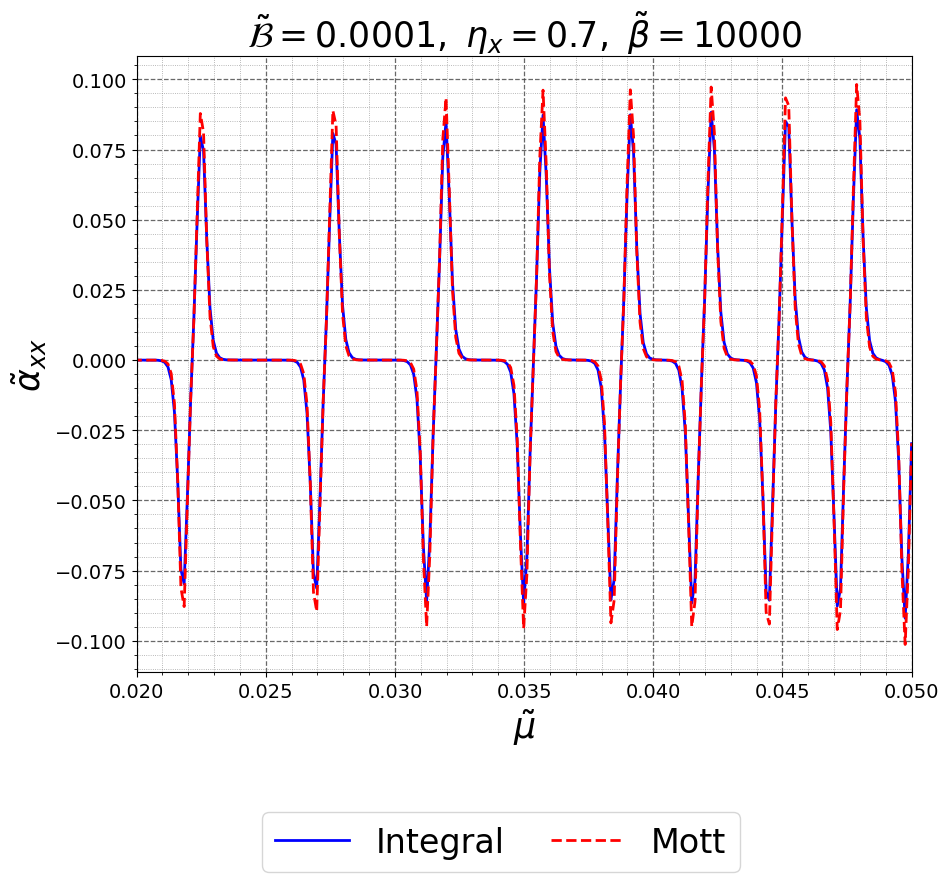
\includegraphics[width=0.425 \textwidth]{mot1}
\hspace{0.3 cm}
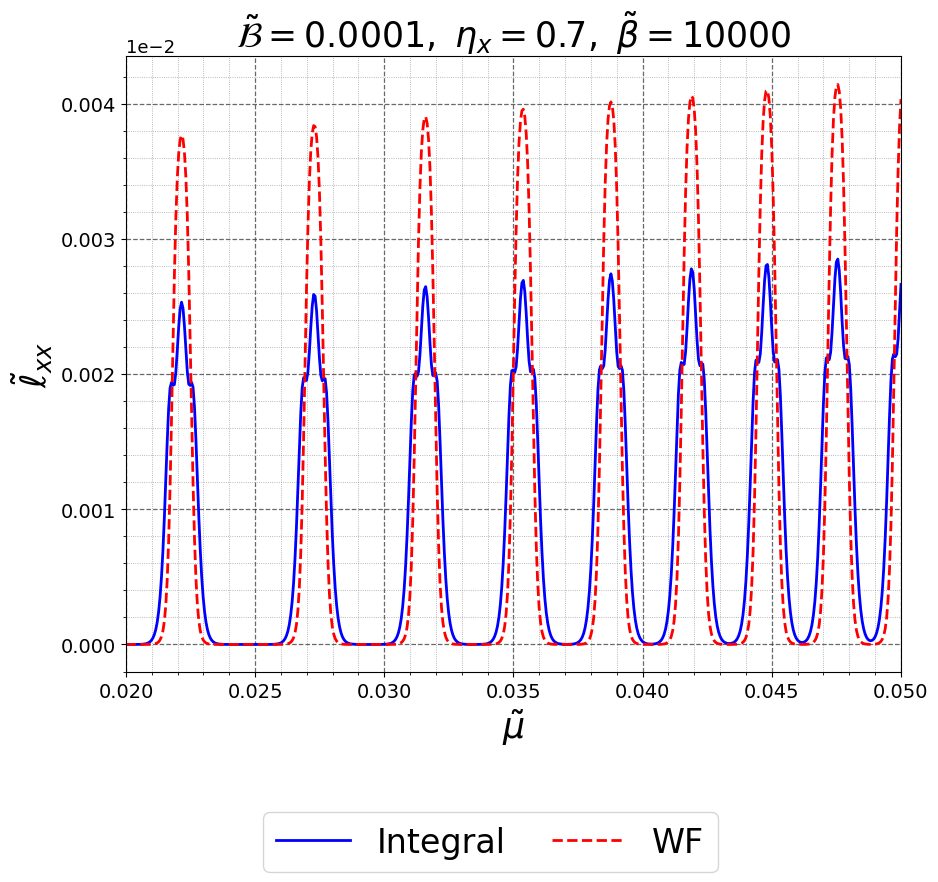
\includegraphics[width=0.42 \textwidth]{mot2} 
\caption{Comparision of the Mott Relation and the Wiedemann-Franz (WF) law [cf. Eq.~\eqref{eqmott}] with the results obtained from the original integrals [cf. Eq.~\eqref{eqalphaell}]. While the blue lines represent the results obtained from the actual integrals (indicated by the label ``Integral''), the dotted red lines show the answers obtained by using the relations. We have used here $v_y/v_x = 0.8$. \rd{The quantities are normalised as in Fig.~\ref{fig:transport}, and the valley is $\xi=+$.} \tbd{Parameters to be completed from the plotting scripts: values of $\tilde{\mathcal B}$, $\eta_x$ and $\tilde\beta$ not stated above. The valley is $\xi=+$.}\label{fig:compare}}
\end{figure*}
%%%%%%%%%%%%%%%%%%%%%%%%%%%%%%%%%%%%%%%%%%%%%%%


Some representative plots, as functions of $\mu$, are shown in Fig.~\ref{fig:transport} for several values of $\beta$. The electrical conductivity demonstrates sharp peaks as a function of $\mu$ --- albeit the peaks get progressively broadened as we go to higher temperatures (i.e., lower values of $\beta$) as the quantised bands of PLLs are exact only at $T = 0$ and a finite value of $T$ smears them out. Due to the extra factor of $(\varepsilon^{{\rm si }}_n - \mu)$ in the integral for $\alpha_{xx}$, compared to that for $ \sigma_{xx}$, each peak-like feature of the $\sigma_{xx}$-curves splits into a pair of asymmetric peaks in the $\alpha_{xx}$-curves. Analogously, due to the extra positive-definite factor of $(\varepsilon^{ {\rm si }}_n - \mu)^2 $ in the integral for $\ell_{xx}$, compared to that for $ \sigma_{xx}$, each peak-like feature of the $\sigma_{xx}$-curves splits into a pair of symmetric peaks in the $ \ell_{xx}$-curves. The response coefficients are asymmetric with respect to $\mathcal B = 0$, which is expected from the explicit forms of the PLLs [cf. Eq.~\eqref{eqevals}].
All these features are distinctly visible for higher and higher $\beta$-values, when thermal smearing gets minimised. 

{\color{red}
All the plotted quantities are dimensionless. Energies are measured in units of $\hbar\,v_x/a_0$, which is about $4.6$ eV for $v_x\simeq10^6$ m/s and $a_0=0.142$ nm, and the temperature follows from $k_{\rm B}\,T=(\hbar\,v_x/a_0)/\tilde\beta$. The quantities $\tilde\sigma_{xx}$, $\tilde\alpha_{xx}$ and $\tilde\ell_{xx}$ are normalised by $\tau$, as defined above, and therefore do not depend on its value. The remaining parameters of each figure are now stated in its caption. The positions of the peaks follow approximately from the band edges of the PLLs. In the absence of tilt, and for small $a_0\,|k_x|$, the peaks recur whenever $\mu^2/(2\,v_x\,v_y\,e\,|\mathcal B|)$ crosses an integer. Their spacing in $|\mathcal B|^{-1}$ is then $2\,v_x\,v_y\,e/\mu^2$, up to corrections from the tilt and from the terms of order $a_0\,k_x$. The peaks are resolved as long as the thermal broadening is smaller than the spacing of the levels, which grows as $\sqrt{|\mathcal B|}$.
}


%%%%%%%%%%%%%
The sensitivity on the values of $\eta_x$ has been depicted via Fig.~\ref{figsigeta}, where $ \delta \sigma \equiv \sigma_{xx}  (\eta_x)/ \sigma_{xx} (\eta_x=0) -1 $ has been plotted. The shifted-parabola shaped curves there show that the dependence has to be fitted with terms $\propto \eta_x$ and those $\propto \eta_x^2 $. At $\mu = 0$, we have unshifted parabolas (i.e., no $\propto \eta_x $ term). A nonzero $\mu$ always gvies a parabola with its vertex shifted away from the origin (towards negative values of both the horizontal and vertical axes) -- the shift increasing with increasing $|\mu|$. We also observe that, lower the temperature, higher the rate of change of the magnitude of $ \delta  \sigma  $ with an increasing $ |\eta_x| $-value.
%%%%%%%%%%
Furthermore, we also illustrate the dependence of the strength of $ \sigma_{xx}$ on $\mathcal B $ through Fig.~\ref{figsigB}. We find that the response falls off rapidly with increasing values of $|\mathcal B |$, which can be traced back to the following: for the realistic values of $\mu $ we have used, the number of PLLs cut by the chemical potential, within a reasonable range of $k_x$ (which is the integration variable), decreases with rising $|\mathcal B|$.

{\color{red}
The dependence on the ratio $v_y/v_x$ enters the spectrum only through $\zeta=e\,\mathcal B\,v_y/v_x$. At leading order, a change of the ratio rescales the level spacing as $\sqrt{v_y/v_x}$ and the upper bound on $n$ as $v_x/v_y$, and it does not change the structure of the response. We have used $v_y/v_x=0.8$ as a representative value of moderate anisotropy. The effects of the strain and of the tilt can be separated in principle. The features that survive at $\eta_x=0$, which include the asymmetry of the response with respect to the sign of $\mathcal B$, are due to the strain, and their sign is reversed by reversing the strain gradient. The contributions $\propto\eta_x$ and $\propto\eta_x^2$ in Fig.~\ref{figsigeta} vanish at $\eta_x=0$, and the linear one is odd under the reversal of the tilt. They are therefore specific to the tilt, and they can be isolated by comparing measurements at two values of the tilt for the same strain profile.
}





Finally, we examine the validity of the Mott relation and the Wiedemann–Franz (WF) law in our strained system, which hold in metallic (or semimetallic) systems for $T  \rightarrow  0 $ in myriad situations \cite{ips-ruiz, ips-rsw-ph, ips-mwsm-floquet}. 
These two relations are captured by
\begin{align}
\label{eqmott}
\partial_{\mu} \sigma_{xx}\,(\mu)
= - \frac{3 \, \textcolor{red}{e}}{T \, \pi^{2}}\, \alpha_{xx} \, (\mu) \,
+ \mathcal{O}\,\left(T^2\right) \text{ and }
%%%%%%%%%%%%
\sigma_{xx}\,(\mu)
= \frac{3 \, e^{2}}{T \, \pi^{2}}\, \ell_{xx}\,(\mu)\,
+ \mathcal{O}\,\left(T^2\right),
\end{align}
respectively.
In conventional metals, these relations hold under the assumption of a smooth energy-dependence of the conductivity near the Fermi level. 
Hence, \textit{a priori}, they are not guaranteed to hold for our case. To check their validity here, we compare the nature of the response-curves obtained by direct computation [via Eq.~\eqref{eqalphaell}] and those obtained from Eq.~\eqref{eqmott}. Such a numerical comparison is demonstrated in Fig.~\ref{fig:compare}, which shows that the relations produce a pretty good fit. 

{\color{red}
The relations in Eq.~\eqref{eqmott} follow from the Sommerfeld expansion of the three integrals in Eq.~\eqref{eqalphaell}, which share the weight $-\partial_\varepsilon f_0\,(\partial_{k_x}\varepsilon)^2$. For an energy-independent $\tau$, they require no further input about the system. They hold when the function
\begin{align}
g(\varepsilon)=\frac{e^2\,\tau}{L_y}\sum_{n,\,{\rm si}}\int\frac{dk_x}{2\,\pi}\,\delta\left(\varepsilon-\varepsilon_n^{\rm si}\right)\left(\partial_{k_x}\varepsilon^{\rm si}_n\right)^2=\frac{e^2\,\tau}{L_y}\sum_{n,\,{\rm si}}\sum_{k_{\rm F}}\frac{|v_x|}{2\,\pi}
\end{align}
varies slowly on the scale of $T$ around $\mu$, with corrections of relative order $(\pi\,T/\delta)^2$, where $\delta$ is the energy scale on which $g$ varies. Here, $g$ is not smooth. Every extremum of a PLL band, and every end point of a branch, changes the number of Fermi points. Near a band minimum, $|v_x|$ grows as the square root of the distance in energy, and $\partial_\varepsilon g$ diverges there. In windows of width of the order of $T$ around these energies, the relations are not controlled. The Wiedemann-Franz law involves $g$ itself and not its derivative, and it is the more robust of the two. Both relations require elastic scattering, and they are exact in the Sommerfeld sense for the constant relaxation time used here. They are consistency checks of the smoothness of $g$, and they do not test the PLL physics itself.

We have quantified the deviations for $\xi=+$, $v_y/v_x=0.8$ and $\eta_x=0.3$ in the window $0.20\le\tilde\mu\le0.40$, restricted to $a_0\,|k_x|\le0.3$. With $\delta_{\rm M}$ and $\delta_{\rm WF}$ denoting the relative deviation, in the sense of the $L^2$ norm over the window, between the direct integral and the right-hand side of the Mott relation and of the Wiedemann-Franz law, respectively, the results are collected in Table~\ref{tabdev}. At fixed $\mathcal B$, the deviation of the Mott relation is of the order of 15 to 20 per cent for temperatures below about a tenth of the level spacing, and it falls below 10 per cent beyond about 0.15 times the spacing. At fixed temperature, it increases with $|\mathcal B|$, because the level spacing grows as $\sqrt{|\mathcal B|}$ and the relation is controlled by the ratio of $T$ to this spacing. Larger pseudomagnetic fields therefore break the Mott relation more strongly at a given temperature, within the range of validity of the continuum model. The Wiedemann-Franz law holds at the level of a few per cent throughout. A larger tilt reduces both deviations, for instance $\delta_{\rm M}=0.14$, $0.12$, $0.08$ and $0.06$ for $\eta_x=0$, $0.15$, $0.3$ and $0.45$ at $\tilde{\mathcal B}=0.01$ and $T=0.004$ (in units of $\hbar\,v_x/a_0$).
 For measurements, this implies that the thermopower at low temperatures cannot be obtained from the gate dependence of the conductivity through the Mott formula and has to be measured directly. The electronic part of the thermal conductivity can be inferred from the conductivity through the Wiedemann-Franz law to the accuracy stated here.
}

\begin{table}[h!]
\centering
{\color{red}
\begin{tabular}{c c | c c c c | c c c c}
\hline\hline
 & & \multicolumn{4}{c|}{$\delta_{\rm M}$} & \multicolumn{4}{c}{$\delta_{\rm WF}$} \\
$a_0^2\,e\,\mathcal B$ & $\Delta E$ & $T=0.001$ & $0.002$ & $0.004$ & $0.008$ & $T=0.001$ & $0.002$ & $0.004$ & $0.008$ \\
\hline
$0.005$ & $0.028$ & $0.175$ & $0.080$ & $0.030$ & $0.009$ & $0.008$ & $0.005$ & $0.004$ & $0.003$ \\
$0.01$ & $0.041$ & $0.164$ & $0.176$ & $0.078$ & $0.028$ & $0.014$ & $0.016$ & $0.009$ & $0.007$ \\
$0.02$ & $0.059$ & $0.147$ & $0.156$ & $0.185$ & $0.077$ & $0.021$ & $0.031$ & $0.036$ & $0.018$ \\
\hline\hline
\end{tabular}}
\caption{\rd{Relative deviations $\delta_{\rm M}$ and $\delta_{\rm WF}$ of the Mott relation and the Wiedemann-Franz law, as functions of $a_0^2\,e\,\mathcal B$ and of the temperature $T$, for $\xi=+$, $v_y/v_x=0.8$, $\eta_x=0.3$ and $0.20\le\tilde\mu\le0.40$. Energies are in units of $\hbar\,v_x/a_0$, and $\Delta E$ is the spacing between the levels $n=1$ and $n=2$ at $k_x=0$.}\label{tabdev}}
\end{table}







\section{Experimental considerations}
\label{secexp}

The calculation is most directly relevant for platforms in which tilted Dirac cones and controllable strain gradients coexist. Strained graphene is the platform in which pseudomagnetic fields have been demonstrated, with pseudo-fields of several hundred tesla in nanobubbles \cite{levy10, graphene-strain-geim, vozmediano10, strain-2d}. A tilt can be induced in the deformed lattice, as discussed in Ref.~\cite{tilted-goerbig}. Organic conductors of the $\alpha$-(BEDT-TTF)$_2$I$_3$ family under pressure host tilted Dirac cones with a large tilt \cite{organic-tilted-dirac}, and the tilt is tunable by the pressure and by its direction. Two-dimensional borophene with tilted anisotropic cones \cite{zhou14} is a further candidate, in which the strain response has still to be explored.

The observables are the following. The first is the longitudinal conductivity as a function of the chemical potential, tuned by a gate, whose peak structure follows the band edges of the PLLs. The second is the dependence of the conductivity on the tilt, $\delta\sigma$ of Fig.~\ref{figsigeta}, which has a term linear in $\eta_x$ for $\mu\neq0$ and no such term at $\mu=0$. The third is the asymmetry with respect to the sign of the pseudomagnetic field, which can be probed by reversing the strain gradient. The fourth is the thermopower $S=\alpha_{xx}/\sigma_{xx}$. By the Mott relation, $S\sim(\pi^2/3)\,(k_{\rm B}/e)\,(k_{\rm B}\,T/\delta)$, which is a few tens of $\mu$V/K for $k_{\rm B}\,T/\delta\sim0.1$ and is within the range of thermopower measurements in graphene.

We estimate the scales as follows. Each Fermi point contributes $e^2\,v\,\tau/(h\,L_y)$ to the conductivity of a valley, that is $e^2/h$ times the ratio of the mean free path to the width. For a mean free path comparable to the width, the contribution of each Fermi point is of the order of $e^2/h\simeq39\ \mu$S, which is well above the resolution of standard transport measurements. The level spacing at $k_x=0$ follows from the Dirac-like ladder, $E_n\simeq\sqrt{2\,n\,v_x\,v_y\,e\,|\mathcal B|}$. For $v_x\simeq v_y\simeq10^6$ m/s, this is about $36\ {\rm meV}\,\sqrt{n\,|\mathcal B|/{\rm T}}$. The PLLs are then resolved at temperatures of a few tens of kelvin for a pseudo-field of about $1$ T. In organic conductors, where the velocities are about an order of magnitude smaller, the spacings are reduced by the same factor. The pseudo-field is related to the strain gradient by $e\,\mathcal B=(\gamma/2)\,\partial_y\varsigma_{yy}$. For $\gamma\,a_0\simeq3$, a strain variation of $1\%$ over $100$ nm corresponds to $|\mathcal B|\simeq0.7$ T. PLL spectroscopy at liquid-helium temperatures \cite{levy10} shows that the disorder broadening in graphene can remain below the spacing of the levels, which is the condition $1/\tau\ll\Delta E$ for the validity of our treatment.

There are practical challenges. The first is the realisation of a strain gradient that is constant over the width of the sample, since the pseudo-field varies if the gradient is not constant. The second is the tuning of the tilt independently of the strain, which in organic conductors is achieved by pressure and which also changes the velocities. The third concerns the valleys. A transport measurement yields the sum of the contributions of both valleys, whereas our figures refer to the valley $\xi=+$. The contribution of the valley $\xi=-$ follows from Eq.~\eqref{eqevals} for $\xi=-$, and it has a different range of the PLLs owing to the strain-induced shift of the Dirac points. The two contributions therefore do not cancel. We do not propose a valley-resolved transport measurement, and the comparison with experiment should be made for the sum. Finally, the strain also shifts the chemical potential, and a gate is needed to separate this effect from that of the PLLs.

\section{Summary and discussion}
\label{secsum}


Contemporary advances in strain-engineering of two-dimensional materials have demonstrated remarkable control over electronic properties via lattice distortions. In particular, theoretical studies suggest that tailored strain in 2d as well as 3d materials can generate pseudomagnetic fields, giving rise to PLLs in the bulk and dispersive edge modes (that reflect the interplay between strain, confinement, and boundary effects). When applied to systems hosting Dirac-like dispersion in their pristine (i.e., unstrained) state, pseudomagnetic fields give rise to valley-dependent transport. The PLLs allow a significant departure from traditional quantum Hall physics, because longitudinal response arises due to the dispersive nature of the bands. The most intriguing feature of the pseudomagnetic field is that we are able to obtain an intrinsic deformation of the bandstructures without actually applying an external magnetic field.


We have focused on the formation of PLLs in tilted Dirac cones, extending the framework of Ref.~\cite{strained-dirac-franz} to incorporate tilt effects and, also, to determine the nature of the electric, thermoelectric, and thermal coefficients. We have calculated the longitudinal components of all the three kinds of response within the semiclassical Boltzmann formalism and have demonstrated their characteristics through representative curves (as functions of the relevant parameters). Our analysis reveals the modifications to expect in linear response, arising from the tilt-parameter. Indeed, if $\eta_x$ can be tuned continuously, it may lead to a mechanically configurable conductance through tilt-controlled residual velocity. Overall, our investigations show how anisotropy (including tilt) modify the  dispersion and transport properties of 2d Dirac-like systems. Our findings contribute significantly to the understanding of strain-engineering in 2d materials and open new pathways for controlling electronic properties through mechanical manipulations, which have potential implications for valleytronic devices and strain-tunable quantum technologies.


\section*{Conflict-of-interest statement}
The authors have no conflicts of interest to declare.

\section*{Data availability}
All data generated or analysed during this study are included in this published article.


%\section*{No funding}

%%%%%%%%%%%%%%%%%%%%%%%%%%

\bibliography{ref_ll}

\appendix
%%%%%%%%%%%%%%%%%%%%%%%%%%

\begin{widetext}
\section*{Appendix: Solving the differential equations}

In this section, we review the derivation of the eigenvalues and eigenvectors of the strained system [defined in Eq.~\eqref{eqhtot}], with a tilt with respect to the $k_x$-axis.
Starting with the Hamiltonian, 
\begin{align}
\label{eqhtotapp}
& \mathcal H_\xi (k_x, y) = \left[ 
 v_x \, \eta_x \, k_x \,  {\mathbb I}_{2\times 2}
 + \mathcal{H}_s(y; k_x, k_y) \right ]\big \vert_{k_y \rightarrow -i\, \partial_y}
\,, \quad 
\mathcal{H}_s  =   d^\xi_x (\bs k)\,\sigma_x +  d^\xi_y (\bs k)\,\sigma_y  \,, \nn &
%%%%%%%%%%%
\frac{ d^\xi_x(\boldsymbol{k}) } {v_x} = \xi \, k_x + s_{-\xi} \, e \, {\mathcal B} \, y\,,
\quad
\frac {d^\xi_y(\boldsymbol{k})} {v_y} =  k_y  \left(s_\xi - r_\xi \, e \, {\mathcal B} \, y\, a_0
\right )  ,
%%%%%%%%%%%%%%
\quad s_\xi = 1 + \frac{\xi \, k_x\, a_0 } {2}\,, \quad
r_\xi = \frac{3}{2} + \frac{\xi \, k_x\, a_0 } {4} \,,
\end{align}
%%%%%%%%%%%%%%%%%%%
we follow the procedure detailed in Refs.~\cite{strained-dirac-franz, complex-LL-strained-graphene}. We solve the eigenvalue equation, $\mathcal H_{\xi=1} (k_x, y) = E\, \Phi (y; k_x)$, by choosing the Dirac-point $D$. 


While dealing with the operators written in the $y$-space, we encounter terms of the form $i\, y\, \partial_y $, which are clearly not Hermiticised. One of the recipes of going from a classical operator (here, $ -i\, y\, \partial_y$) to its quantum version is symmetrisation, which we apply here (following Ref.~\cite{strained-dirac-franz}). Let us denote $y$ by $\check y$ and $-i\, \partial_y$ by $\check k_y$ to explicitly indicate that these are the position and momentum operators along the $y$-direction, projected into the position-space representation. Then we must replace any occurrence of $ -i\, y \,\partial_y $ by
$$ \frac{\check{y} \,\check{k}_y}{2}  +   \frac{\ \check{k}_y \, \check{y} }{2} = \check{y} \,\check{k}_y + \frac{1}{2} \,.$$
Going back to our original notation, we just replace $ -i\, y \,\partial_y $ by $-i\left ( y\,\partial_y + 1/2 \right)$ in the final expressions. After eliminating $\phi_A$ using the two equations arising from the two spinor components and shifting the $y$-coordinate as $ y\rightarrow y + 
\frac{s_+}{r_+ \,a_0\,  e\, {\mathcal B}}$, the final equation for $\phi_B$ turns out to be
%%%%%%%%%%%%%%%%%%%%%%%%%%%%
\begin{align}
\label{eqdiffea}
& \left[(s_{-}\,e \, {\mathcal B}\,y)^2 + \frac{s_{-} \,e \, {\mathcal B}}{\tilde{r}}(2\,k_x\,\tilde{r}+2\,s_{-}\,s_+
-e \, {\mathcal B}\,\tilde{r}^2)\,y+\frac{\Delta}{\tilde{r}^2}-\frac{\zeta^2\,\tilde{r}^2}{4} \right] \, \phi_B 
-2 \,y \, \zeta^2 \, \tilde{r}^2 \, \partial_y \phi_B-y^2 \, \zeta^2 \, \tilde{r}^2 \, \partial^2_y \phi_B = 0\,,
%%%%%%%%%%%%
\nn & \tilde{r} = a_0 \, r_+ \,, \quad \zeta =  e \, {\mathcal B} \, \frac{v_y}{v_x} \,, \quad
\epsilon = a_0 \, \left( \frac{E}{v_x}- \eta_x \, k_x \right), \quad
\Delta = (k_x \, \tilde r+ s_{-} \, s_+ )^2-\tilde r^2 \, \epsilon^2 \,.
\end{align}
%%%%%%%%%%%%%%%%%%%
%For nonzero $\eta_y$, there are imaginary terms which necessitate taking $\phi_B $ to be complex, which we parametrise as 
%$ \phi_B(y) = A_\phi (y) + i \,B_\phi (y)$. Taking the real and imaginary parts, we arrive at
%%%%%%%%%%%%%%%%%%
%\begin{align}
%& \left[(p_+ \,b\,y)^2+\frac{ p_+ \, b\, y} {r_+ } \left (2\,k_x\,r_+ +2 \, p_+ \, s-b\,r_+^2 \right )
%+\frac{\Delta}{r_+^2}-\frac{b^2\,r_+^2}{4}
%-\frac{1}{4}   \right] A_\phi 
%-\left (2 \,y \, b^2\, r_+^2 + 2\,y \right ) \partial_y A_\phi
%\nn & -\, y^2 \left (b^2 \,r_+^2+1 \right ) \partial^2_y A_\phi 
%+ \epsilon \,\eta_y \, B_\phi  
%+ 2\,y \,\epsilon \,\eta_y\, \partial_y B_\phi = 0 \,, \nn
%%%%%%%%%%%%%%%%%%%%%%
%& \left[( p_+ \,  b\, y)^2 + \frac{ p_+ \,  b\, y } {r_+ } \left (2 \,k_x\,r_+ + 2\, p_+ \, s-b\,r_+^2 \right )
%+\frac{\Delta}{r_+^2}-\frac{b^2 \,r_+^2}{4}-\frac{1}{4}\right]B_\phi
%-\left (2 \,y \,b^2 \,r_+^2 + 2\,y \right ) \partial_y B_\phi
%-y^2 \left (b^2 \,r_+^2+1  \right ) \partial^2_y B_\phi \nn &
%-\epsilon \eta_y \, A - 2\,y \,\epsilon \eta_y\,\partial_y A_\phi =0 \,.
%\end{align}
%%%%%%%%%%%%%%%%%%%
%These are coupled equations in $A_\phi$ and $B_\phi$, which make analytical solutions unfeasible. Hence, we consider the simpler case with $\eta_y = 0$ and solve for real $\phi_ B $ , as considered in Refs.~\cite{tilted-goerbig-plasmons, strained-dirac-franz}.
%%%%%%%%%%%%%%%%%%%%%%%%%%
The above form is in the form of a Sturm-Liuouville (SSL) problem, viz. $\partial_y \left[ \mathcal P (y)\,\partial_y \phi_B \right ] - \, {\mathcal Q} (y)\,\phi_B = -\,\lambda\, {\mathcal W}(y)\,\phi_B $. In fact, it is a singular SSL scenario because the interval $(-\infty, 0]$ (or, $ [0, \infty)$) infinite and ${\mathcal P} (y) = 0$ at the boundary $y= 0$. Next, we perform an asymptotic analysis of the system at $y\rightarrow0$ and $ |y| \rightarrow \infty$ Ref.~\cite{strained-dirac-franz}:
%%%%%%%%%%%%%%%%%%%
\begin{itemize}
\item For $y\rightarrow0$, the leading-order terms reduce to
\begin{align}
\left[\frac{\Delta}{\tilde{r}^2}-\frac{\zeta^2\,\tilde{r}^2}{4} \right] \, \phi_B 
-2 \,y \, \zeta^2 \, \tilde{r}^2  \, \partial_y \phi_B- \zeta^2 \, \tilde{r}^2 \,y^2 \, \partial^2_y \phi_B=0 \,,
\end{align}
which has solutions going as $\phi_B \sim y^{-\frac{1}{2}\pm{\frac{\sqrt{\Delta}}{\tilde{r}^2 \, |\zeta|}}} $. The $y=0$ regime represents one with regular singularity. The only physically-admissible solution is  $ \phi_B \sim y^{-\frac{1}{2}+{\frac{\sqrt{\Delta}}{\tilde{r}^2 \, |\zeta|}}} $, since the other one diverges. \rd{Physically, this selects the wave function that vanishes at $y=0$, which is the point where the coefficient of $k_y$ in $d^\xi_y$, that is the strain-reduced velocity along $y$, vanishes after the shift of the coordinate.} 

\item For $ |y| \rightarrow\infty$, we need to solve for
\begin{align}
\left (s_{-}\,e \, {\mathcal B}\,y \right )^2  \phi_B -y^2 \,\zeta^2 \, \tilde{r}^2 \, \partial^2_y \phi_B=0 \, ,
\end{align}
which has the solution of the form, $ y \sim \exp \left [ {\pm \, e\, |{\mathcal B}|  \,s_- \; y} /(\tilde r \, \zeta) \right ] $. 
Each solution diverges either at $ y = \infty$ or $y=-\infty $ and, hence, none is physically admissible along the entire $y$-axis. These points are therefore irregular singularities.

\end{itemize}
%%%%%%%%%%%%%%%%%%%%%
Knowing the forms of the asymptotic expressions, we now take the ansatz Ref.~\cite{strained-dirac-franz} (suppressing the explicit $k_x$-dependence),
% \\\textcolor{red}{here}
\begin{align}
\phi_B (y) = e^{-\tilde y/2} \, 
y^{-\frac{1}{2}+{\frac{\sqrt{\Delta}}{\tilde{r}^2 \, |\zeta|}}} \,  u(y) \,,\quad
%%%%%%%%%%%%%%
\tilde y = -\, \frac{ 2\, v_x \, \text{sgn} (\mathcal B) \,s_-} { v_y \,\tilde r }\, y \,.
\end{align}
%%%%%%%%%%%%%%% 
Changing variables from $y$ to $\tilde y $ and defining $\tilde u(\tilde y) = u(y)$,
we end up with a confluent hypergeometric differential equation for $\tilde u(\tilde y)$, away from the singularity [considering the interval to be either $(-\infty, 0]$ or $ [0, \infty)$], which can be expressed as
\begin{align}
& {\tilde y}\, \partial^2_{\tilde y} \tilde u (\tilde y)
+ (\Gamma- \tilde y)\, \partial_{\tilde y} \tilde u({\tilde y})-\alpha \,\tilde u({\tilde y}) = 0\,, \quad
\alpha = \frac{\tilde r^2 \, (e \, {\mathcal B}+|\zeta|)+ 2 \, (\sqrt{\Delta}-s_{-} \, s_+ -k_x \, \tilde r)} 
{2 \, |\zeta| \, \tilde r^2} \,, \quad
%%%%%%%%%%%%%%%%%%%%
\Gamma = 1+ \frac{2 \,\sqrt{\Delta }}{\tilde  r^2 \, |\zeta|}\, .
\end{align}
%%%%%%%%%%%%%%%%%%%%%%
It turns out that the regular solutions involve the Kummer’s function, $\mathcal M (\alpha, \Gamma, \tilde y)$, where $\alpha = - n $ (taking $n \in 0 \cup {\mathbb{Z}}^+ $) is a non-positive integer but $\Gamma $ is not. Then, we have the condition that
\begin{align}
-\,n = \frac{\tilde r^2 \, (e \, {\mathcal B}+|\zeta|)+ 2 \, (\sqrt{\Delta}-s_{-} \, s_+ -k_x \, \tilde r)} 
{2 \, |\zeta| \, \tilde r^2} 
%%%%%%%%%%%%
\Rightarrow
\sqrt{\Delta}=-\tilde r^2 \, |\zeta |\, n+k_x \, \tilde r-\frac{\tilde r^2}{2}
(e \, \mathcal B+ |\zeta|)+s_{-} \, s_+ \,.
\end{align}
%%%%%%%%%%%%%%%%%%%%%%%%%%%%%
Using the relation $ \Delta = (k_x \, \tilde r+s_{-} \, s_+ )^2-\tilde r^2 \, \epsilon^2 $, it leads to
\begin{align}
\epsilon^2 = \tilde r^2 \, \left( |\zeta |\, n + \frac{e \, \mathcal B+ |\zeta|}{2} \right)^2
+ \left (k_x \, \tilde r+s_{-} \, s_+ \right ) \left (2 \, |\zeta |\, n + e \, \mathcal B+|\zeta| \right),
%%%%%%%%%%%%%
\quad \mathcal M (-n, \Gamma, \tilde y) = {\mathcal L}^{\Gamma-1}_{n}(\tilde y)\,,
\end{align}
where ${\mathcal L}^\ell_{n} (\tilde y )$ is the Generalized (or, alternatively, Associated) Laguerre polynomial with $ n \in 0 \cup {\mathbb Z}^+$. \rd{The condition $\alpha=-n$ truncates the series of the confluent hypergeometric function to a polynomial, which is the analogue of the Landau quantisation condition. The integer $n$ counts the nodes of the wave function along $y$, and the dependence of $\sqrt\Delta$ on $k_x$ through $\tilde r_\xi$ and $s_\xi$ is what makes the levels dispersive.} Imposing the requisite physical condition that $\epsilon^2 \geq 0 $, we obtain an upper bound for $n$ as $ 
\left\lfloor\frac{8 \,(2  + 3 \, \xi \,a_0\, k_x)}   { a_0^2\,|\zeta| \,(6 +\xi \,a_0\,  k_x)^2} \right\rfloor  $. The symbol $\left \lfloor  \Upsilon \right \rfloor$ denotes the greatest integer less than or equal to $\Upsilon$. The final solution is obtained as Ref.~\cite{strained-dirac-franz}
\begin{align}
& \phi_B (k_x, y+ y^+_{\rm sg}) \, \Theta \left[ \text{sgn}(\mathcal B ) \left(- y\right)  \right],\,
\text{ where }\nn
%%%%%%%%%%%%%%%%%%%%
 &\phi_B (k_x, y) = e^{\frac{  v_x \, \text{sgn} (\mathcal B) \,s_{-\xi}\, y} { v_y \, r_+\, a_0 }} \, 
y^{-\frac{1}{2}+{\frac{ v_x \,\sqrt{\Delta}}{ r_\xi^2\, a_0^2\, e  \, v_y  \left |{\mathcal B}  \right |}}} \, 
{\mathcal L}^{\Gamma-1}_{n}(\tilde y)\,, 
%%%%%%%%%%%%%
 \quad  y^+_{\rm sg} = \frac{s_+ } {r_+ \,a_0\,  e\, {\mathcal B}}\,,\quad
\tilde y = -\, \frac{ 2\, v_x \, \text{sgn} (\mathcal B) \,s_-} 
{ v_y \,r_+\, a_0 } \, y \,.
\end{align}
%%%%%%%%%%%%%%%%%%%%%%%%%
Clearly, the full wavefunction does not diverge at the irregular singularity, as it is cut-off by the Heaviside-theta function and it goes to zero before reaching that singular point.



The same process can be repeated for the valley with $\xi =- $. Using $E= \frac{v_x} {a_0} \left[  \eta_x \,   k_x + \epsilon   \right ]$, we finally get the PLLs as
%%%%%%%%%%%%%%%%%%%
\begin{align}
\frac{  E^{\xi}_{n, \rm{si}} (k_x, \mathcal B) } {v_x} =  
\eta_x \,   k_x + \text{si} \,
\sqrt{\tilde r_\xi^2 \, \left( |\zeta | \, n
+ \frac{e \, \mathcal B+|\zeta|}{2} \right)^2
+ \left (k_x \, \tilde r_\xi + s_{-\xi} \, s_\xi \right )
\left (2 \, |\zeta |\, n + e \, \mathcal B+|\zeta| \right )}  \,,
\text{ where } \tilde{r}_\xi = a_0 \, r_\xi \text{ and } \text{si} =\pm\,.
\end{align}
%%%%%%%%%%%%%%%%%%%%%%%%
We have labelled them by the integer-index $n$, momentum $k_x$, and band-index $\pm$ at the valley $\xi$. The valley-dependent wavefunction, for the $n^{\rm th}$ PLL, is captured by
\begin{align}
& \phi_B^{\xi,n, \text{si}} (k_x, y+ y^\xi_{\rm sg}) \, \Theta \left[ \text{sgn}(\mathcal B ) \left(- y\right)  \right],\,
\quad
%%%%%%%%%%%%%%%%%%%%
 \phi_B^{\xi, n, \text{si}} (k_x, y) = e^{\frac{ v_x \, \text{sgn} (\mathcal B) \,s_{- \xi}\, y} { v_y \, r_\xi\, a_0 }} \, 
y^{-\frac{1}{2}+{\frac{ v_x \,\sqrt{\Delta}}{ r_\xi^2\, a_0^2\, e  \, v_y  \left |{\mathcal B}  \right |}}} \, 
{\mathcal L}^{\Gamma-1}_{n}(\tilde y)\,, 
\quad  \Gamma = 1+ \frac{2 \,\sqrt{\Delta }}{\tilde  r_\xi^2 \, |\zeta|} \,,\nn
%%%%%%%%%%%%%
& \quad  y^\xi_{\rm sg} = \frac{s_\xi } {r_\xi \,a_0\,  e\, {\mathcal B}}\,,\quad
\tilde y = -\, \frac{ 2\, v_x \, \text{sgn} (\mathcal B) \,s_{-\xi}\, y} 
{ v_y \,r_\xi \, a_0 }\,, \quad
%%%%%%%%%%%%%%%%%%%
\sqrt{\Delta}=-{\tilde r}_\xi^2 \, |\zeta |\, n + k_x \, {\tilde r}_\xi -\frac{\tilde r_\xi^2}{2}
(e \, \mathcal B + |\zeta|)+s_{\xi} \, s_{-\xi} \,.
\end{align}
%%%%%%%%%%%%%%%%%%%%%%%%%
We also show below the explicit expression for the upper component of the $n^{\rm th}$-PLL's eigenspinor, $ \Phi^{\xi, n, \text{si}} (k_x, y) = \begin{bmatrix}
\phi_A^{\xi, n, \text{si}}  (k_x, y) && \phi_B^{\xi, n, \text{si}}  (k_x, y)  \end{bmatrix}^T $:
%%%%%%%%%%%%%%%%%%%%%%%%%%%%
\begin{align}
\label{eqphia}
& \phi_A^{\xi, n, \text{si}} (k_x, y)  =  \frac{1}{v_x} \frac{
e^{\frac{2v_x \,\mathrm{sgn}(\mathcal{B})\, s_{-\xi}\, y}{v_y\, r_\xi\, a_0}}
\, y^{-\frac{3}{2} + 
\frac{v_x \sqrt{\Delta}}{r_{\xi}^2\, a_0^2\, e\, v_y\, \left|\mathcal{B}\right|}}
\left[
{\mathcal{F}}_1^\xi\,\mathcal{L}_{n}^{\Gamma-1}(\tilde{y})
-
{\mathcal{F}}_2^\xi \,\mathcal{L}_{n-1}^{\Gamma-1}(\tilde{y})\right]}
{ \frac{ E^{\xi}_{n, \rm{si}} (k_x, \mathcal B)} {v_x} - \eta_x \,   k_x }\,,
%%%%%%%%%%%%%%%%%%%%%%%%
\nn & {\mathcal{F}}_1^\xi   = 8 \, v_x  \, F_1^\xi  \, F_2^\xi + 8 \,  r_\xi
\left [ 4 \,v_y|\mathcal{B}|\,r_\xi\,F_3^\xi 
+ 8  \, \mathcal{B} \, v_x \,  y\,F_4^\xi  \right ],\quad
%%%%%%%%%%%%%%%%%%%%%%%%%%
{\mathcal{F}}_2^\xi  = 256\, v_x\, y\, |\mathcal{B}|\, r_\xi
\left[a_0 \,\mathcal{B} \,y \,r_\xi + v_y \left (s_\xi-2 \right )\right]
(s_\xi-2)\, \text{sgn}(\mathcal{B})\,,
\end{align}
where
\begin{align}
F_1^\xi  &=  2 \, \mathcal{B}  \, r_\xi^2 + a_0^2 \,  k_x^2 \left (1 - \xi \right )
-6 \, a_0  \, k_x - 4\,, \quad
%%%%%%%%%%%%%%%%%%
F_2^\xi  = 4 \, a_0 \, \mathcal{B} \, y  \, r_\xi + 4 \, v_y\left (s_\xi-2 \right ), \nn
%%%%%%%%%%%%%%%%%%%%
F_3^\xi  &= 4\,v_y \left (n+1 \right ) \left (s_\xi-2 \right ) 
+k_x  \,  \xi \,y \left[ a_0^3  \, \mathcal{B}\,(n+1)-4 \, v_x\right]
+6 \, a_0^2 \, \mathcal{B}\,(n+1)\,y\,, \nn
%%%%%%%%%%%%%%%%%%%
F_4^\xi  & = y\, r_\xi \left(4 \,a_0\,\mathcal{B}\,s_\xi-8\,a_0 \, \mathcal{B}
+ a_0 \,\xi\, v_y-2\, v_y \right)
+ 4\,v_y\left(s_{-\xi} \, s_\xi-1\right).
\end{align}


\end{widetext}



 
\end{document}
